%%%%%%%%%%%%%%%%%%%%%%%%%%%%%%%%%%%%%%%%%%%%%%%%%%%%%%%%%%%%%%%%%%%%%%%%%%%%%%%
%%  claude-giga-lens-linus --- SECTIONS C (P5 report build).
%%
%%  Contents: (1) the sampler decision matrix (benchmark results),
%%            (2) calibration gifts + handoff package,
%%            (3) discussion,
%%            (4) reproducibility (ledgers, budget, environment freezes).
%%
%%  Every number below is quoted from research/synthesis_tables.md (the spine),
%%  whose seven DISCREPANCY FLAGS are binding: where an on-disk artifact and the
%%  CAMPAIGN.md prose disagree, the ARTIFACT value is quoted, with the flag
%%  noted in place. Compatible with the claude-giga-lens report preamble
%%  (../../tech-report.sty + the main.tex macro block: \gammaEPL, \Rhat, \ESS,
%%  \art, \dfile, ...).  Bright lines (PLAN \S8) bind this text: the team's
%%  repositories are referenced only as ``the upstream development branches,''
%%  their unpublished results are not characterized, and the carousel data use
%%  is acknowledged as data provided by the team, used with permission, with
%%  comparison deferred pending sign-off.
%%%%%%%%%%%%%%%%%%%%%%%%%%%%%%%%%%%%%%%%%%%%%%%%%%%%%%%%%%%%%%%%%%%%%%%%%%%%%%%

% Local shorthands (providecommand: safe if the preamble or a sibling section
% already defines them).
\providecommand{\sboot}{\ensuremath{\sigma_{\mathrm{boot}}}}
\providecommand{\sseed}{\ensuremath{\sigma_{\mathrm{seed}}}}
\providecommand{\logZ}{\ensuremath{\log Z}}
\providecommand{\dlogZ}{\ensuremath{\Delta\log Z}}
\providecommand{\mcsmc}{prior-seeded MAMS-SMC}

%%%%%%%%%%%%%%%%%%%%%%%%%%%%%%%%%%%%%%%%%%%%%%%%%%%%%%%%%%%%%%%%%%%%%%%%%%%%%%%
\section{The Sampler Decision Matrix}
\label{sec:matrix}
%%%%%%%%%%%%%%%%%%%%%%%%%%%%%%%%%%%%%%%%%%%%%%%%%%%%%%%%%%%%%%%%%%%%%%%%%%%%%%%

The benchmark's deliverable is not a ranking but a {\it decision matrix}: for
each target class that a lens modeler actually faces, which inference vehicle
converges, which yields trustworthy evidence, and at what cost. Four vehicles
were exercised under the frozen P0 protocol: {\bf S1}, cold-start
\mcsmc\ (tempered SMC with Metropolis-adjusted microcanonical mutations,
adaptive $\lambda$-schedule, per-stage bootstrap \logZ); {\bf warm MAMS}, a
MAP-warm-started MAMS-alone arm (no tempering); {\bf MCLMC-mutation SMC},
formally demoted to a diagnostic at the B0 correctness gate (below) and never
used as an evidence kernel; and the {\bf classic} MAP$\to$SVI$\to$HMC baseline
recipe at frozen single-stage settings. Table~\ref{tab:decision} is the full
matrix; the subsections that follow give each row's evidence and the two
cross-cutting findings. Every cell is pre-registered (design checkpoint with
derived thresholds logged before submission) and closed in the final gate
ledger (\S\ref{sec:repro}). The per-fit convergence diagnostics behind
every cell --- one row for each fit the campaign ever ran, including the
failed, rejected, and budget-blocked arms --- are tabulated in
Appendix~\ref{app:convergence}.

\begin{table}[tbp]
\centering
\caption{The sampler decision matrix. Rows are target classes; columns are
vehicles. ``---'' = not run (pre-registered scope, budget close, or
prerequisite unmet; dispositions in
\dfile{research/gate\_ledger\_final.md}). All A100 costs are actual
ledgered hours. The carousel row uses real MUSE cutouts provided by the team,
used with permission; comparison against the team's own runs is deferred
pending sign-off. The DSPL and easy-scene target builders come from the
upstream development branches (used with permission). Scene-substrate
cells are proposed (UNCERTIFIED --- external): reproduced/measured on
the vendored scene API, with certification belonging to the receiving
team.}
\label{tab:decision}
\scriptsize
\setlength{\tabcolsep}{3.5pt}
\renewcommand{\arraystretch}{1.3}
\begin{tabular}{@{}p{0.145\textwidth}p{0.23\textwidth}p{0.115\textwidth}p{0.13\textwidth}p{0.145\textwidth}p{0.13\textwidth}@{}}
\toprule
target class & S1 \mcsmc & warm MAMS & MCLMC (demoted) & classic MAP$\to$SVI$\to$HMC & evidence yield \\
\midrule
{\bf T0 analytic} (2-d bimodal; funnel-10; illcond-46) --- B0, 0 A100-h &
mix2 {\bf PASS} (\logZ\ err 0.073); funnel10 {\bf FAIL} $-0.66$ nat (class
limitation, reproduced in the old validated stack); illcond46 {\bf PASS}
worst-$z$ 1.83 but \logZ\ err 2.40 nat $=6.6\sboot$ &
--- (an HMC-mutation SMC arm ran as comparison) &
{\bf DEMOTED}: \dlogZ\ vs MAMS $+10.79\pm0.54$ $=20.1\sigma$ on illcond46 &
n/a &
analytic refs; \sboot\ provably understates \logZ\ error (finding A) \\
{\bf easy scene} 22-d unimodal $\times4$ --- B3, free tier, 0 A100-h &
{\bf BLOCKED-BY-BUDGET} 0/4 inside the 5\,h/arm L4 fence at $N{=}512$; the
readable result is the cost row &
--- & --- &
4/4 complete but 0/4 pass the frozen acceptance rule
($\Rhat_{\rm worst}$ 4.36--7.87) $\Rightarrow$ {\bf BLOCKED-BY-REFERENCE} &
none (no accepted posterior on either arm) \\
{\bf DSPL thin ridge} 21-d --- B2/B2$'$, 2.9 A100-h &
$\lambda{=}1$ @64 stages, sanity clean; $\hat m$ 0/512 vs.\ imported band
$\Rightarrow$ falsifier control shows the band is realization-specific;
B2$'$ {\bf PASS-UNDERPOWERED} &
--- & --- & --- &
\dlogZ(orig$-$ratio) $=+3.06\pm0.35_{\rm boot}$ where true $\Delta\approx0$
(finding A, measured) \\
{\bf T2} 46-d cond-$10^{14}$ --- B4 + arbitration, 4.4 A100-h &
healthy but wall-capped $\times3$ (A100 $\lambda{=}0.587$ @3.5\,h; L4
$\lambda{=}0.418$ at a 12.3-h resume leg) $\Rightarrow$ {\bf
budget-infeasible}; B4 itself not evaluable within budget &
(the classic arm was warm-started) & --- &
{\bf NO-VERDICT}: $\Rhat_{\rm worst}$ 44.3, all chains railed
$\gammaEPL\approx1.99$ --- the known T2 single-stage pathology, reproduced
cross-stack &
none; premise carried by likelihood parity + the L0-G2 row \\
{\bf T3} 74-d bimodal --- B5, 1.9 A100-h (+1.7 infra) &
{\bf G1 PASS both basins} ($\lambda{=}1$, retention 1.000);
{\bf G2 FAIL-as-written} $11.0\sigma$ --- decomposition indicts our own
frozen reference's within-basin coverage (finding B) &
--- &
{\bf G3 AMBIGUOUS}: minor-mode evidence inflated $\times56$; within-basin
$\gammaEPL$ untouched &
--- &
occupancy robust across all estimators; absolute \logZ\ NOT robust at the
$\pm5$-nat gate scale \\
{\bf carousel} 33-d multi-plane, real --- B1r, 15.85 A100-h &
$\lambda{=}0.1506$ @36 stages after 11.33\,h, {\bf 0 posterior samples}
(sampler healthy; killed by cost) &
budget-matched S6br: wall fence in burn round 11/30, {\bf 0 draws},
$\ESS{=}0$ at 41.5\% of the grad budget &
--- & --- &
none --- {\bf NEITHER CONVERGES}; the cost row is the deliverable \\
{\bf v3b correlated}, real, 46-d --- L0-G2, 0.53 A100-h &
{\bf PASS}: $\gammaEPL$ $\Delta$ 0.0027, \logZ\ $\Delta$ 0.11 nat
cross-stack; \dlogZ(steep$-$low) in the seed family &
--- & --- & --- &
best evidence row of the campaign; correlated port licensed \\
\bottomrule
\end{tabular}
\end{table}

\begin{figure}[tbp]
\centering
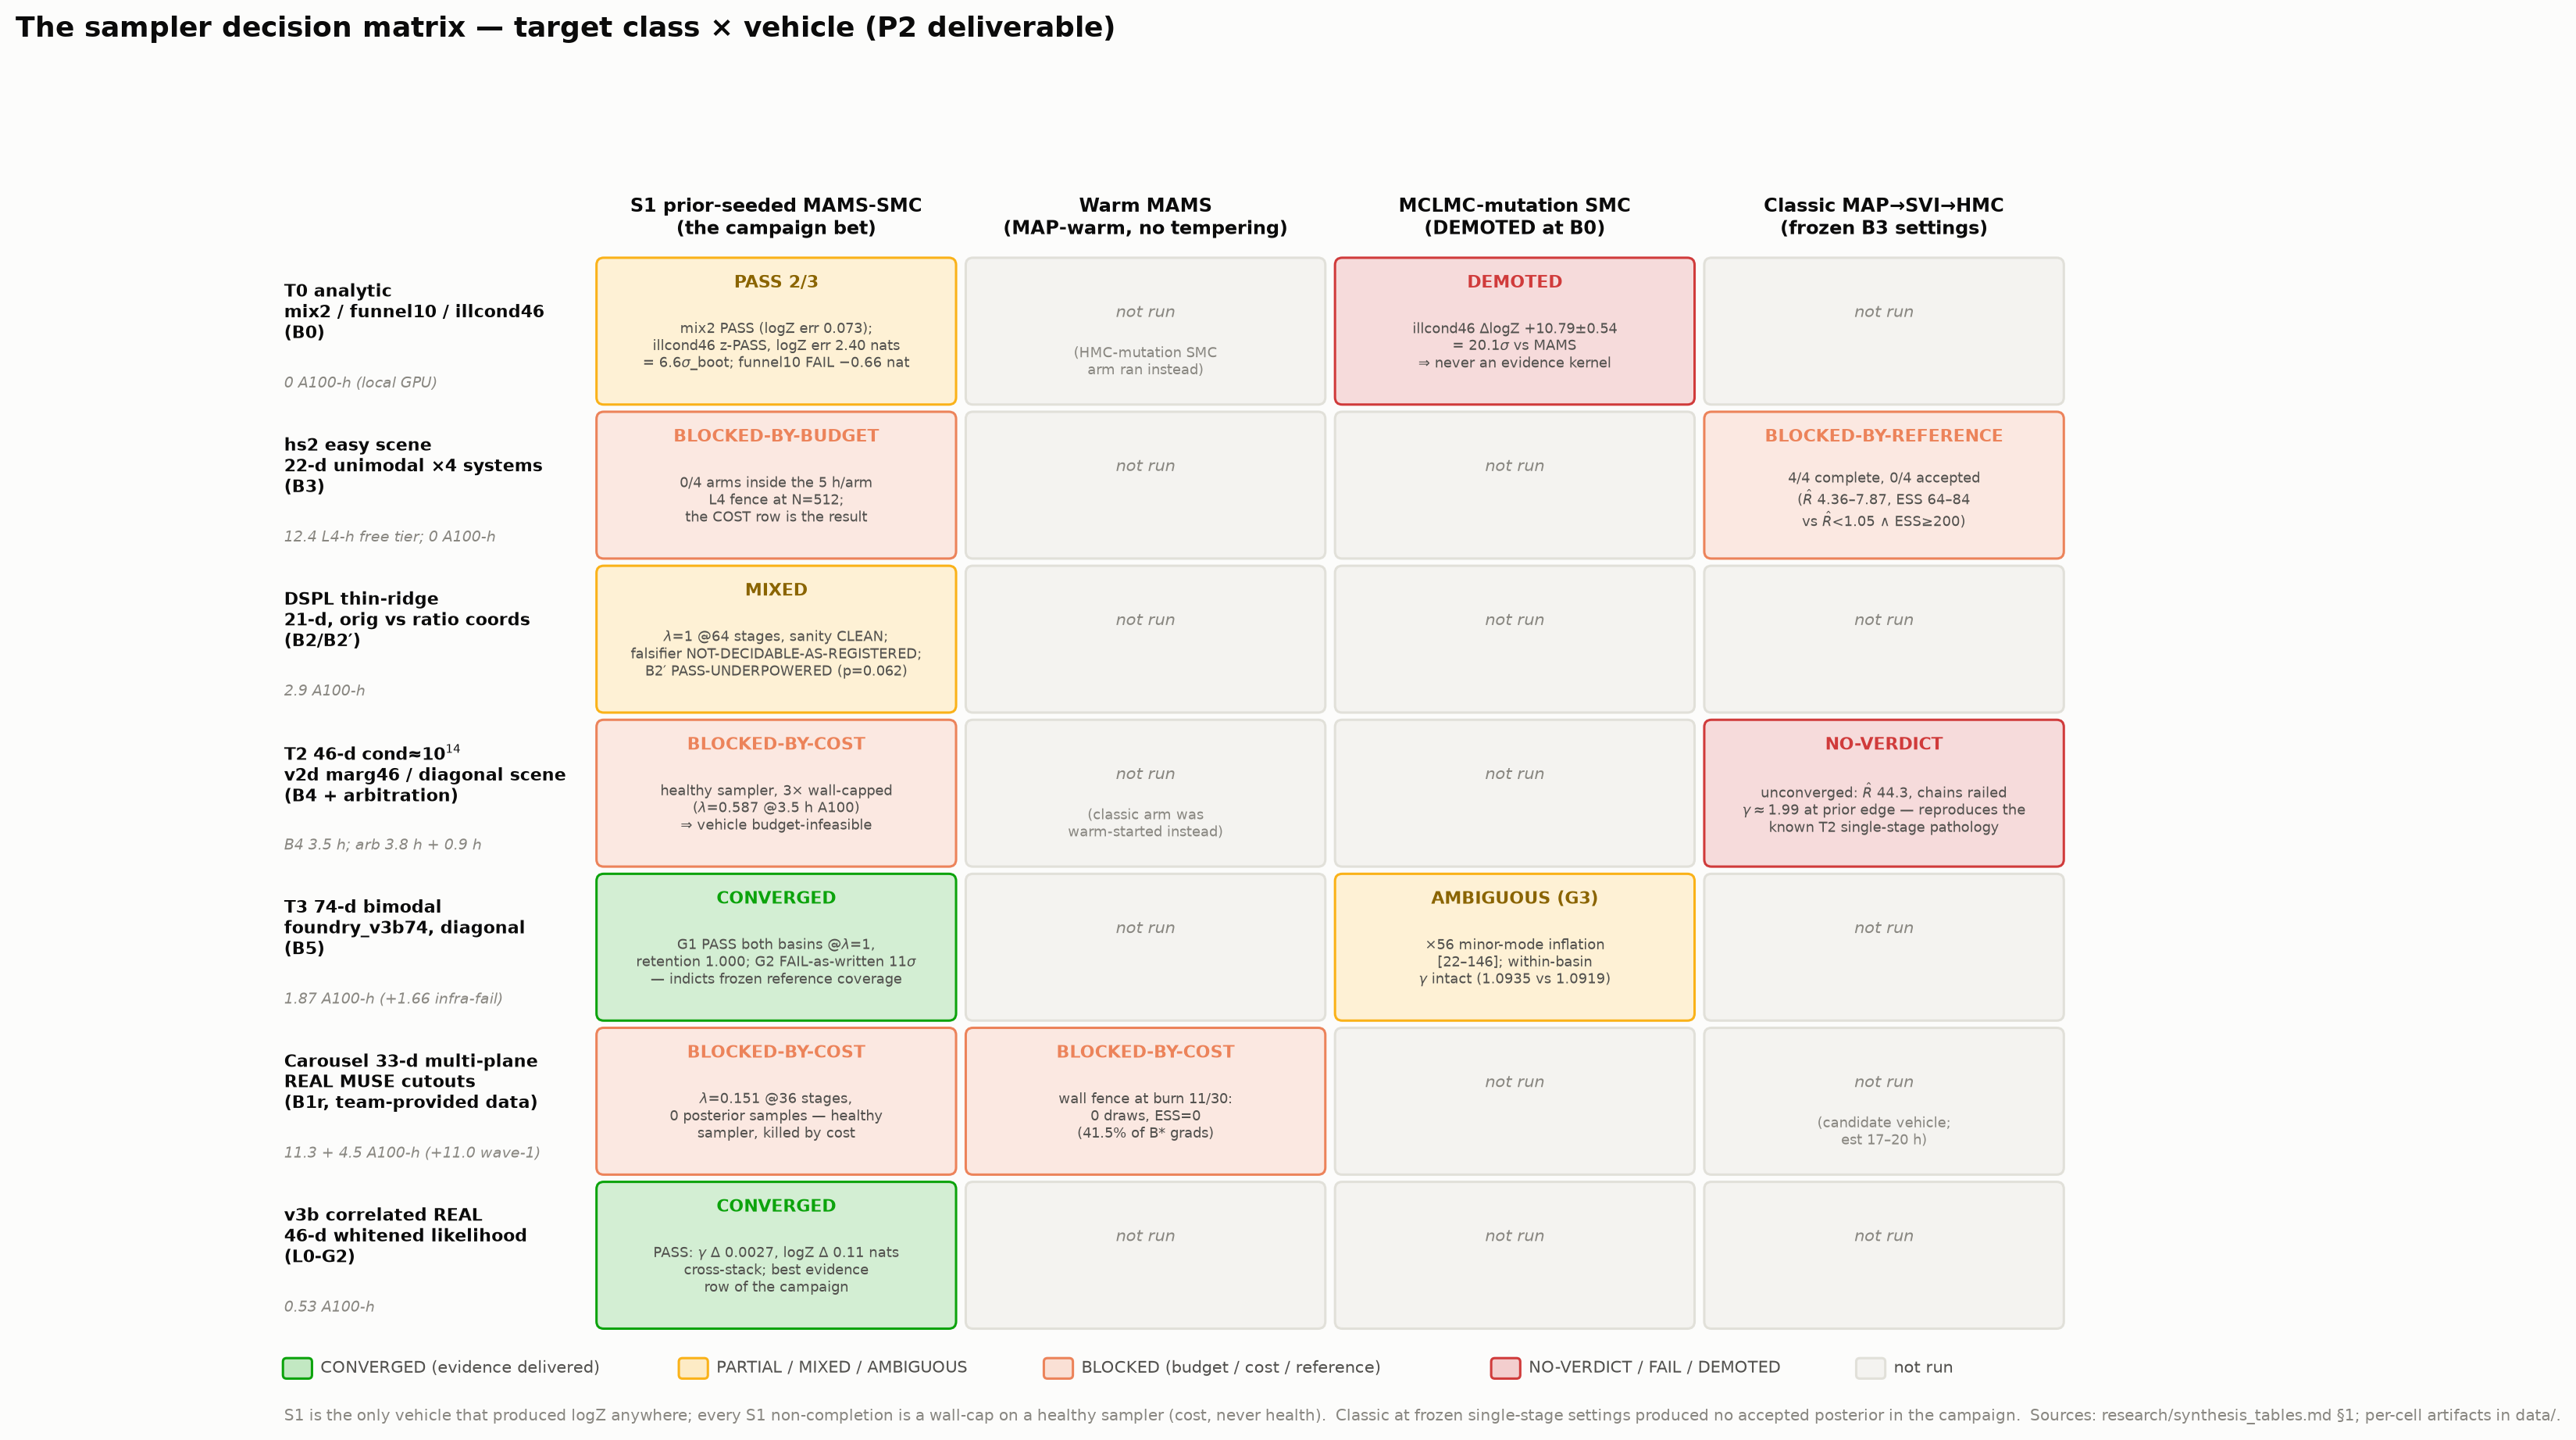
\includegraphics[width=0.99\textwidth]{../figs/rfig_decision_matrix.png}
\caption{The sampler decision matrix as a capability grid (the graphical
form of Table~\ref{tab:decision}): 7 target classes $\times$ 4 vehicles.
Cell status is the gate-ledger final disposition (green = converged with
evidence delivered; yellow = partial/mixed/ambiguous; salmon = blocked by
budget, cost, or reference; red = no-verdict/fail/demoted; gray = not
run), with the discriminating measurement and the realized cost in each
run cell. The honest reading is baked in: S1 \mcsmc\ is the only vehicle
that produced \logZ\ anywhere; every S1 non-completion is a wall-cap on a
healthy sampler; the classic recipe at frozen settings produced no
accepted posterior; MCLMC was demoted at B0 ($\dlogZ=+10.79\pm0.54 =
20.1\sigma$, artifact value) and stayed diagnostic-only. Sources:
\dfile{research/synthesis\_tables.md} \S1;
\dfile{research/gate\_ledger\_final.md}; per-cell artifacts as cited in
Table~\ref{tab:decision} and the subsections.}
\label{fig:matrixfig}
\end{figure}

\subsection{Reading the matrix: measured capability boundaries}
\label{sec:matrix:boundaries}

Three boundaries are measured, not conjectured. First, {\bf \mcsmc\ works ---
converges {\it and} yields evidence --- on analytic targets, the DSPL ridge,
the 74-d bimodal target (both basins, retention 1.000), and the correlated
real-data v3b refit}; it is the only vehicle in the campaign that produced
\logZ\ at all. Second, {\bf when it fails, it fails by cost, never by
health}: every non-completion (B1 mocks, B1r real carousel, B3 at $N{=}512$,
the three arbitration wall-caps) is a wall-clock cap on a sampler whose
per-stage diagnostics were clean at the kill point ---
$\lambda$-progress per A100-hour is the binding constraint on scene-substrate
real targets. Third, {\bf the classic single-stage recipe produced zero
accepted posteriors in this campaign} (B3 0/4, the arbitration arm's
NO-VERDICT, and 30/32 unhealthy fits in the X2 SBC arm at reduced budget) ---
consistent with the prior campaign's finding that this posterior family needs
the two-stage re-preconditioned recipe; its unique value here was diagnostic
(\S\ref{sec:matrix:classic}).

\subsection{Carousel (B1r): neither vehicle converges at campaign budget}
\label{sec:matrix:b1r}

The carousel cell is the campaign's designated hard real-data row: a 33-dim
multi-plane model on real MUSE cutouts (data provided by the team, used with
permission; any comparison against the team's own runs is deferred pending
their sign-off). The cold-start arm S1r ($N{=}128$, three chained
checkpointed legs) spent 11.33 A100-h to reach $\lambda=0.1506$ at 36 stages
--- {\it zero} posterior samples, with the sampler demonstrably healthy at
the fence (92--104 unique particles of 128, acceptance 0.871--0.934), so
$\lambda=1$ is infeasible under any campaign-scale
budget.\art{data/results-perlmutter/b1r128\_carousel33\_s1\_seed2.PARTIAL.json}
The pre-registered close-out framing was written {\it before} the baseline
ran, including the branch that would have scored against our own bet (``any
nonzero baseline \ESS\ $\Rightarrow$ decisive cold-start LOSS''). That branch
did not fire: the warm MAMS-alone baseline S6br, budget-matched at S1r's
realized $3{,}078{,}912$ gradient evaluations, hit its 4.5-h wall fence in
burn round 11 of 30 --- {\bf sampling never started} (0 draws, $\ESS=0$,
\Rhat\ not computable) at $1{,}277{,}632$ grads $=41.5\%$ of the budget,
with burn itself healthy (acceptance 0.873--0.902).\art{data/b1r\_decision\_matrix.json}
Per-gradient throughput agrees across arms to $\sim$5\% ($\sim$284k vs.\
272k grads/h), so the truncation is a {\it target-cost} fact, not arm
inefficiency. The row's honest verdict: {\bf carousel-class real targets are
out of reach for both vehicles at these budgets} (an until-converged warm
arm is estimated at 17--20\,h from the wave-1 anchors, untested). The
descoped gates (2-seed self-consistency, \logZ\ repeatability) remain
descoped and are stated as such in the amendment of
record.\art{research/checkpoint\_b1r\_close.md}

\begin{figure}[htbp]
\centering
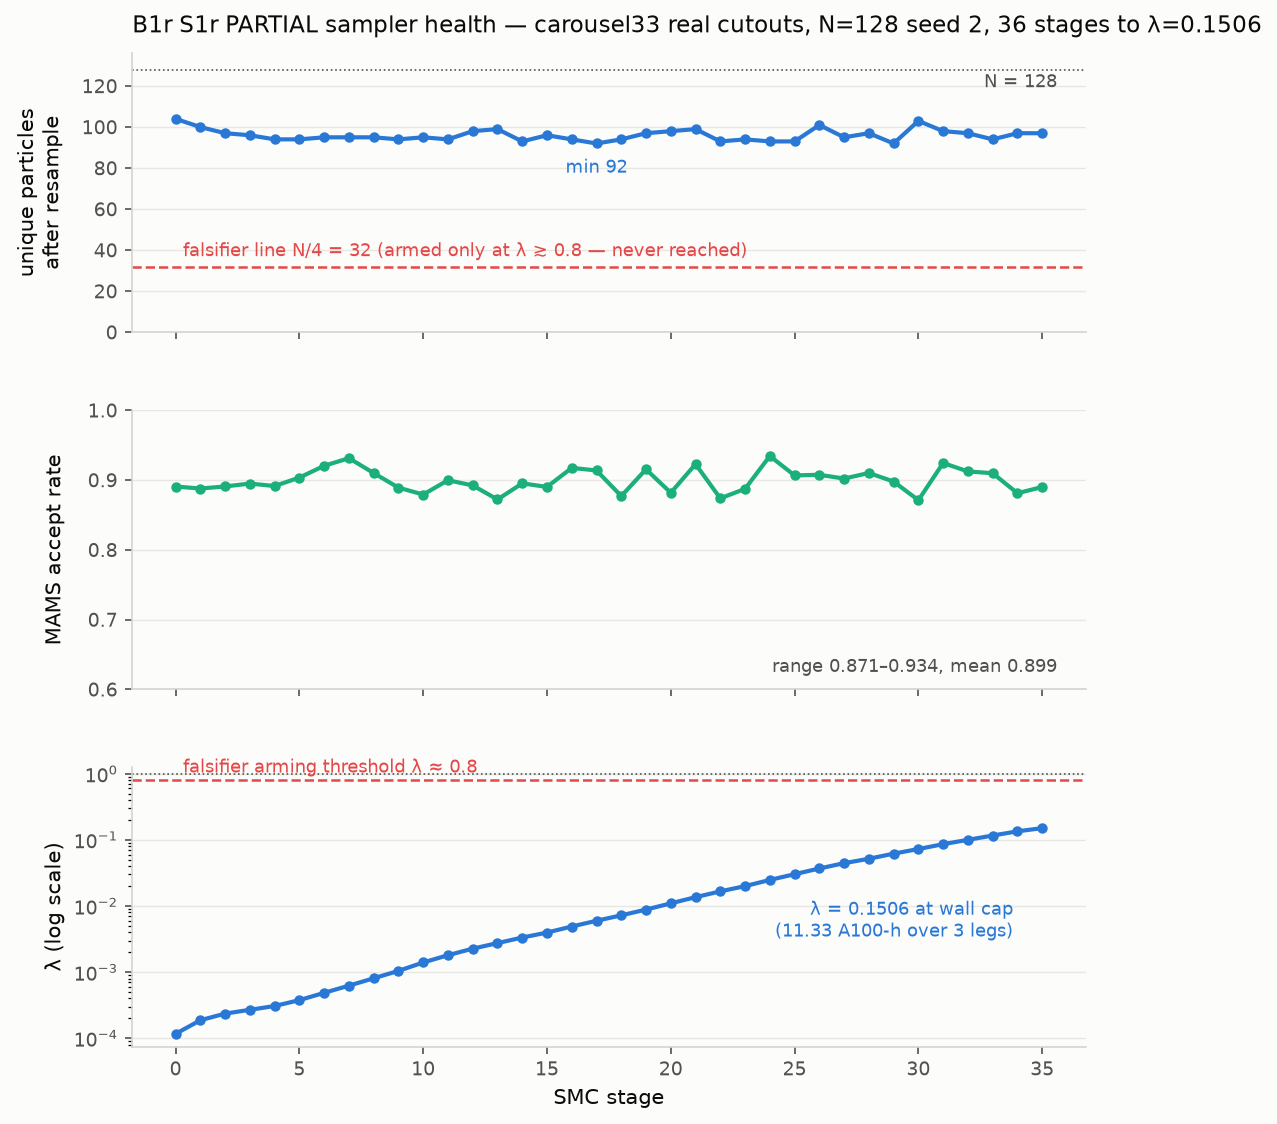
\includegraphics[width=0.58\textwidth]{../figs/b1r_s1_partial_traces.png}\\[4pt]
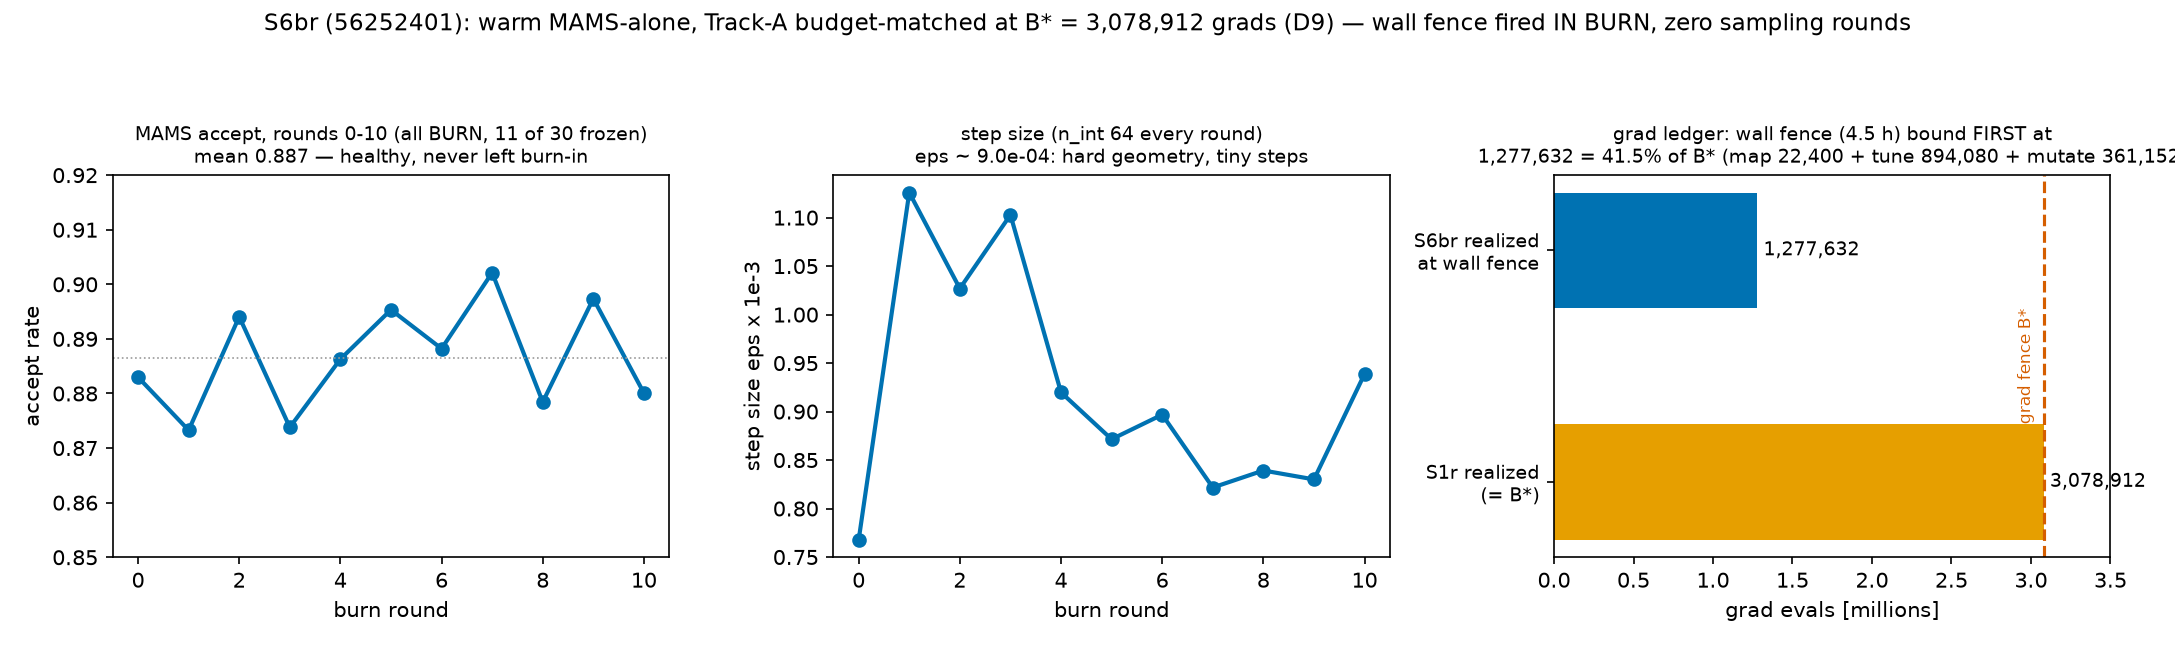
\includegraphics[width=0.94\textwidth]{../figs/b1r_s6br_traces.png}
\caption{The carousel cell B1r (real MUSE cutouts provided by the team,
used with permission; comparison with the team's own runs deferred
pending sign-off); both panels plotted before gate text per house rule.
Top: the S1r cold-start MC-SMC arm over three chained checkpointed legs
to $\lambda=0.1506$ at 36 stages (11.33 A100-h) --- unique-particle
counts 92--104 of 128 and acceptance 0.871--0.934 at the fence: a
healthy sampler killed by cost. Bottom: the budget-matched warm-MAMS arm
S6br (job 56252401) hits its 4.5-h wall fence in burn round 11 of 30 ---
sampling never started ($\ESS=0$ at $1{,}277{,}632$ grads $=41.5\%$ of
the matched $3{,}078{,}912$-gradient budget), with burn itself healthy.
Sources:
\dfile{data/results-perlmutter/b1r128\_carousel33\_s1\_seed2.PARTIAL.json};
\dfile{data/b1r\_decision\_matrix.json}.}
\label{fig:b1r}
\end{figure}

\subsection{T3 bimodal (B5): both basins pass; the gate that fails indicts
our own frozen reference}
\label{sec:matrix:b5}

On the 74-d bimodal target, S1 delivers the multimodality certificate {\bf
G1} in full: the low basin reaches $\lambda=1$ in 31 stages (retention
1.000, $\gammaEPL_{\rm eqw}=1.0919$, $\logZ=38376.33\pm0.33_{\rm boot}$) and
the steep basin in 22 stages ($\gammaEPL_{\rm eqw}=2.5552$,
$\logZ=38518.23\pm0.31_{\rm boot}$).\art{data/b5\_gate\_eval.json}

\begin{figure}[htbp]
\centering
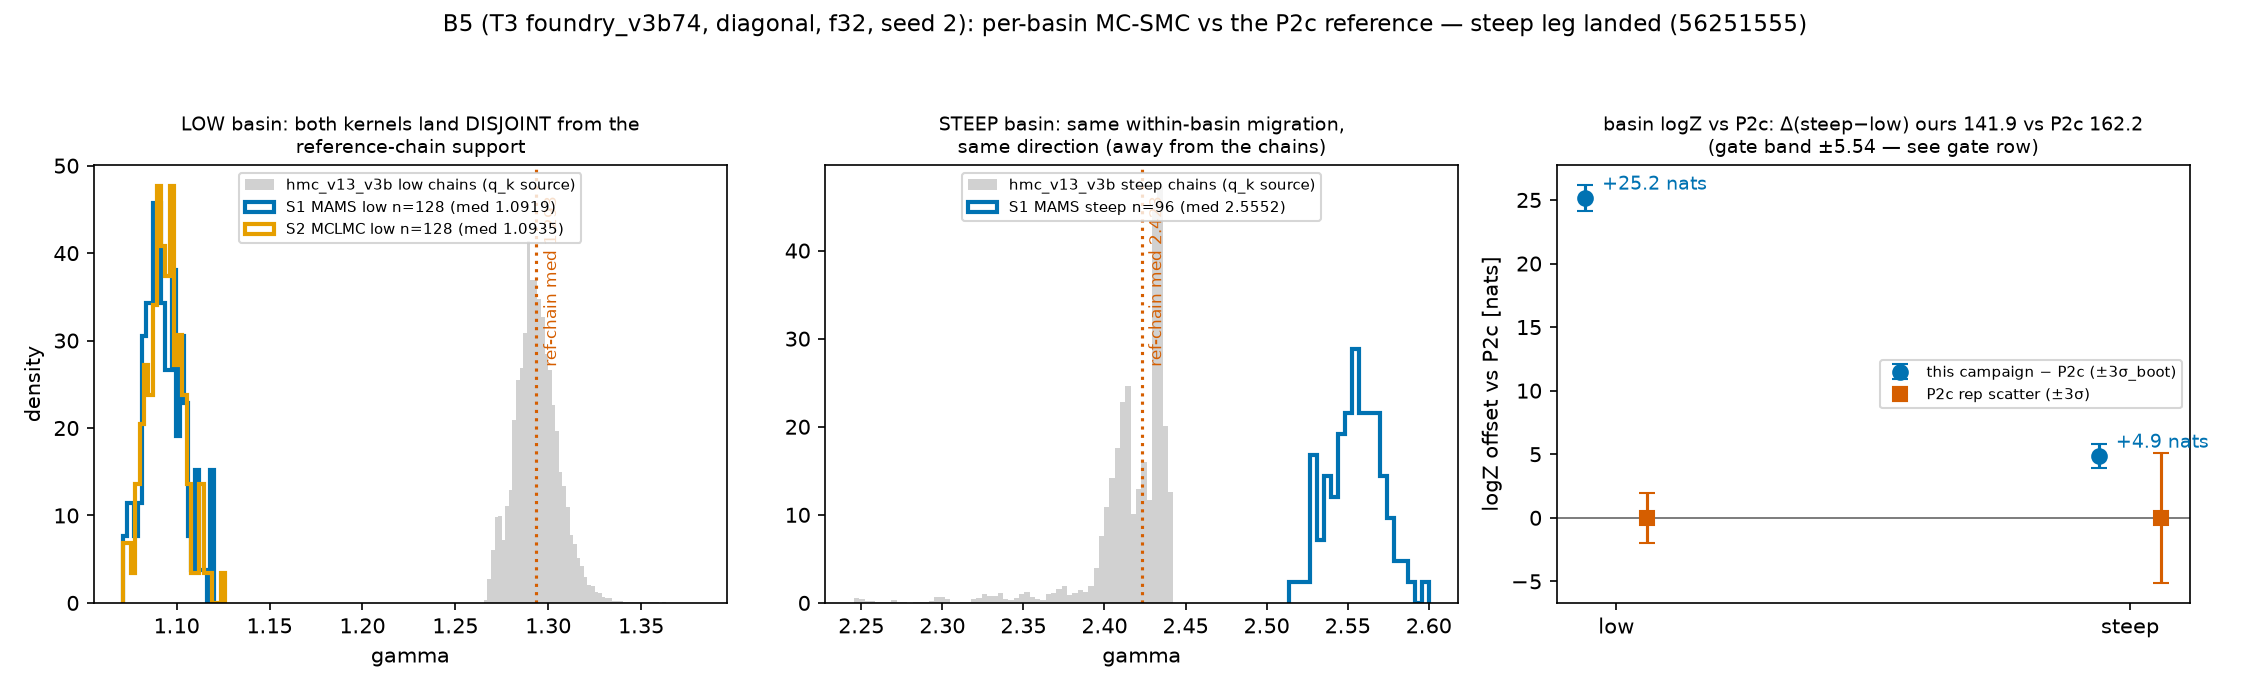
\includegraphics[width=0.92\textwidth]{../figs/b5_basin_overlay.png}
\caption{B5 both-basin $\lambda=1$ posterior overlay on the 74-d bimodal
target \dfile{foundry\_v3b74}, drawn \emph{before} any gate math per
house rule (jobs 56006049 / 56251555 / 56006052). The low basin's two
independent mutation kernels agree on location (MAMS
$\gammaEPL_{\rm eqw}=1.0919$, MCLMC 1.0935); the steep basin sits at
2.5552. Source: \dfile{data/b5\_gate\_eval.json}.}
\label{fig:b5overlay}
\end{figure}

{\bf G2} --- basin \dlogZ\ against the frozen per-basin evidence reference
from {\it our own previous campaign} (P2c) --- {\bf fails as written}, by a
lot: $\Delta(\mathrm{steep}-\mathrm{low}) = +141.90\pm0.45$ vs.\ the
reference $+162.2\pm1.8$, a $-20.30$-nat miss against a $5.54$-nat band
($11.0\times$ the gate $\sigma$-scale). We frame this carefully, because the
honest decomposition cuts {\it toward the reference}: the per-basin offsets
are $+25.16$ (low) and $+4.86$ (steep) --- {\it both} basins carry {\it
more} evidence than the reference, in the same direction --- and both
$\lambda=1$ ensembles are $\gammaEPL$-{\it disjoint} from the fixed-step HMC
chains the reference was seeded and mutated from (low basin: ours
$[1.071,1.126]$ vs.\ chains $[1.265,1.381]$), with two {\it independent}
mutation kernels agreeing on the location (MAMS 1.0919, MCLMC 1.0935). The
adaptive anneals reach higher-log-probability shelves that the reference's
short fixed-step chains never visited. Comparability was verified line by
line before scoring (same target constructor, identical evidence
construction, the importance weights cancel; the reference's own on-disk
smoke reproduces its $\Delta=162.7$ under its kernel), so the discrepancy is
real --- and with $n{=}1$ seed on the measuring side, final attribution
between reference and vehicle is explicitly undecidable within the closed
budget. What the fail {\it does} establish is cross-cutting finding B
(\S\ref{sec:matrix:crosscutting}): frozen MCMC-derived evidence references
can carry within-basin coverage error far exceeding the gate scale. This is
a statement about our own prior artifact, not about any external one.

{\bf G3}, the pre-registered MCLMC-laundering probe, lands {\bf ambiguous at
the frozen thresholds} because its two frozen clauses conflict on the
measured value: the diagnostic MCLMC arm inflates minor-mode evidence by
$+4.03\pm0.49$ nats $=\times56$ $[\mathrm{CI}_{95,\rm boot}\ 22\text{--}146]$
--- $8.3\sboot$ from zero and $6.0\sboot$ above the pre-registered
$1.5$--$3\times$ ceiling, so SMC resampling does {\it not} launder the
unadjusted-MCLMC bias at point estimate --- yet the shift sits inside the
imported 5.56-nat \sseed\ repeatability band, so the laundering falsifier
technically fires. Within-basin location is untouched
($\gammaEPL$ 1.0935 vs.\ 1.0919): the bias lands in the evidence, not the
posterior. Either way the physical conclusion is robust across every
estimator: the minor mode is negligible ($w_{\rm low}\le1.3\times10^{-60}$
in all constructions), while {\it absolute} evidence calibration at the
$\pm5$-nat gate scale is not.

\begin{figure}[htbp]
\centering
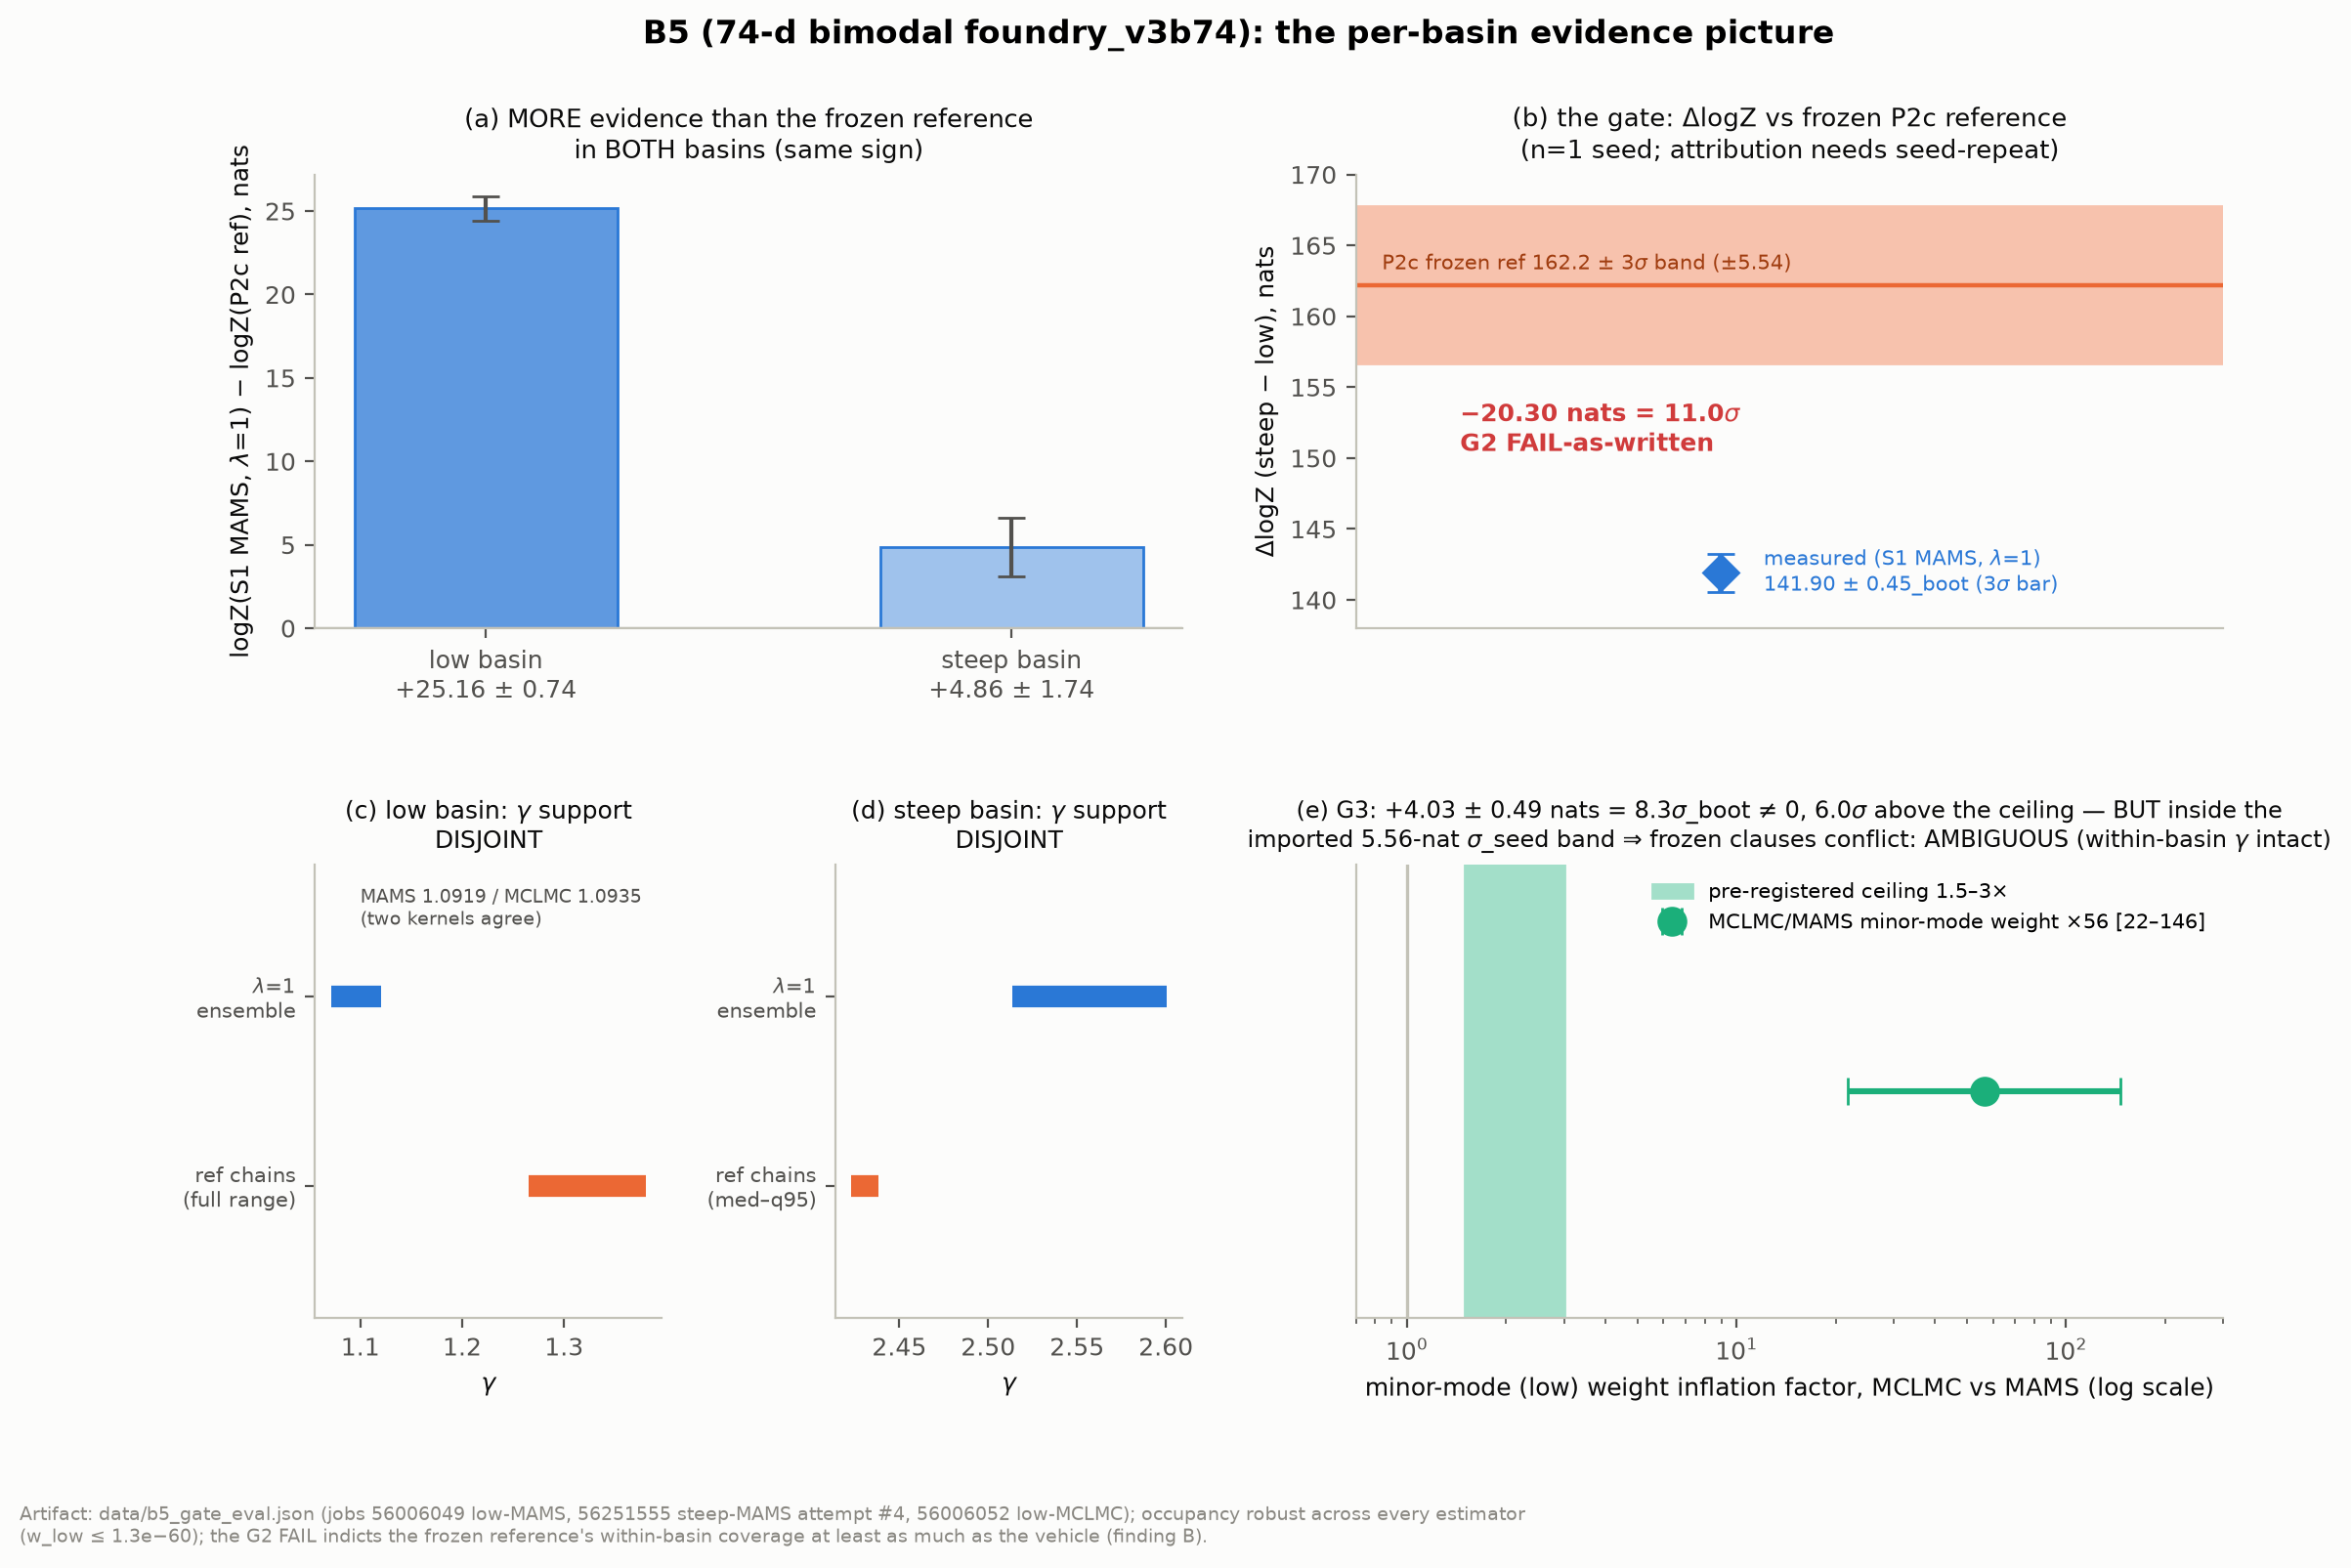
\includegraphics[width=0.98\textwidth]{../figs/rfig_b5_evidence.png}
\caption{B5 per-basin evidence picture on the 74-d bimodal target.
(a) The S1 $\lambda=1$ ensembles find \emph{more} evidence than the
frozen P2c reference in \emph{both} basins ($+25.16\pm0.74$ low,
$+4.86\pm1.74$ steep --- same sign). (b) The G2 gate as written
therefore fails at $11.0\sigma$ (measured
$\Delta=141.90\pm0.45_{\rm boot}$ vs.\ reference $162.2\pm1.8$, band
$\pm5.54$~nats) --- but the decomposition in (a) plus (c,d) indicts the
frozen reference's within-basin coverage at least as much as the
vehicle: both $\lambda=1$ ensembles are $\gammaEPL$-disjoint from the
reference-chain support that the reference was seeded \emph{and} mutated
from, while two independent kernels (MAMS 1.0919, MCLMC 1.0935) agree on
the low-basin location (cross-cutting finding B; $n{=}1$ seed,
attribution undecidable within the closed budget). (e) The MCLMC
diagnostic arm inflates minor-mode evidence $\times56$
[$\mathrm{CI}_{95,\rm boot}$ 22--146] $=+4.03\pm0.49$~nats ---
$6.0\sboot$ above the pre-registered $1.5$--$3\times$ ceiling yet inside
the imported 5.56-nat \sseed\ repeatability band, so the two frozen G3
clauses conflict: AMBIGUOUS, and the B0 demotion stands. Minor-mode
occupancy is robust across every estimator
($w_{\rm low}\le1.3\times10^{-60}$). Source:
\dfile{data/b5\_gate\_eval.json} (jobs 56006049, 56251555 attempt \#4
chunk-32, 56006052; frozen P2c reference constants therein).}
\label{fig:b5}
\end{figure}

\subsection{DSPL (B2/B2$'$): the realization-calibration lesson}
\label{sec:matrix:b2}

The DSPL thin-ridge cell was scored twice, and the sequence is the lesson.
As written, B2 asked S1 (in the original, deliberately pathological
coordinates) to recover a pre-registered minor-arm mass band
$0.103\pm0.045$, imported at design time. The measured $\hat m = 0/512$
fails the band --- but the pre-registered falsifier control, an {\it exact}
reparameterization of the same posterior on the same data (which cannot
suffer coordinate mode-death), measures this realization's true arm mass at
$5/512 = 0.0098\pm0.0043$, itself far outside the band.\art{data/b2\_gate\_eval.json}
The band does not transfer across data realizations; the gate was
{\bf not decidable as registered}, and the pre-registered branch mandated
re-registration rather than silent re-scoring. The re-registered B2$'$
(rule and attainable-significance clause declared before scoring) compares
the arms directly: two-sided Fisher $p=0.0619 \ge \alpha=0.01$ ---
{\bf PASS-UNDERPOWERED (consistent)}, with the honest caveat that with only
five minor-arm particles in total no outcome could have failed at $\alpha$;
minor-arm under-coverage up to $\sim\times3$ is not excluded (the one-sided
signal, $p=0.031$, is $\sim2\sigma$ and suggestive at most). The dominant
arm is statistically identical across coordinates ($\Omega_{m,0}$ median
0.4701 vs.\ 0.4702). The headline stands at ``no detected coordinate
pathology'' strength --- and the cell's most valuable by-product is an
evidence-error datum: $\dlogZ(\mathrm{orig}-\mathrm{ratio}) =
+3.06\pm0.35_{\rm boot}$ nats on identical data where the exact
reparameterization forces the true $\Delta\approx0$
(\S\ref{sec:matrix:crosscutting}).

\begin{figure}[htbp]
\centering
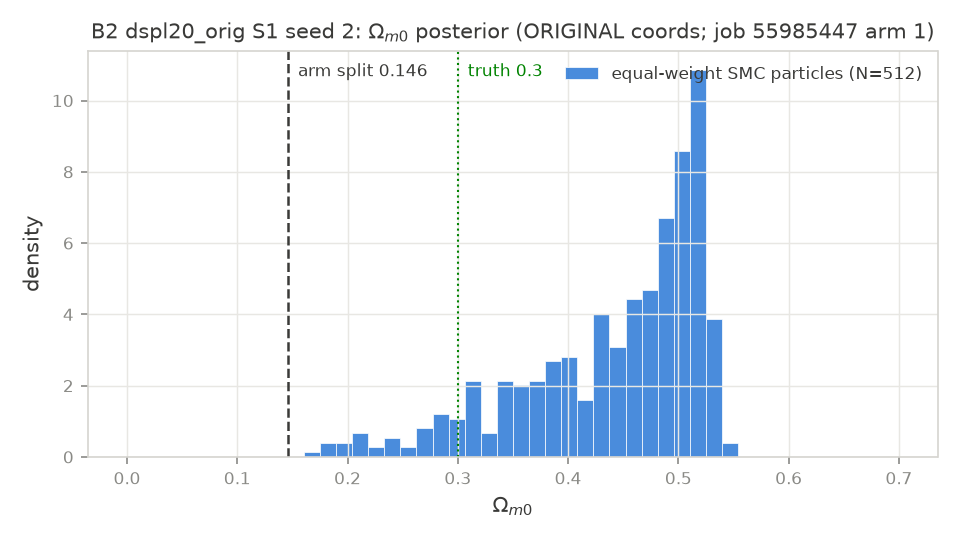
\includegraphics[width=0.37\textwidth]{../figs/b2_om0_posterior.png}\hfill
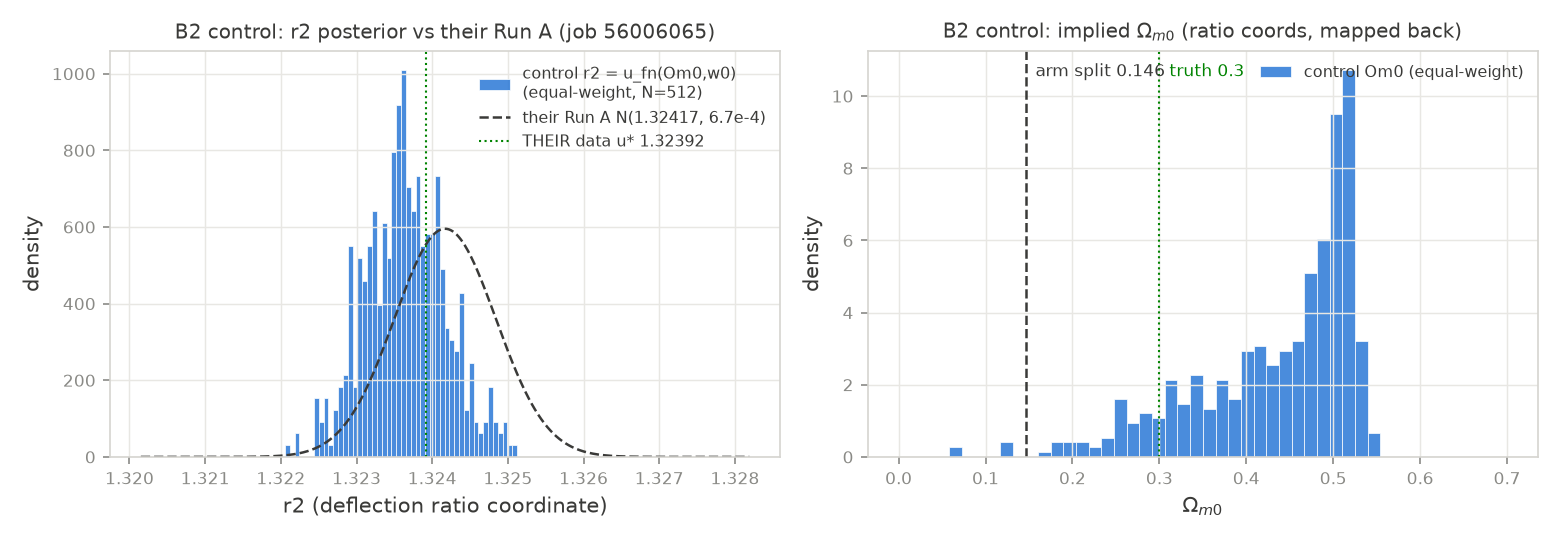
\includegraphics[width=0.60\textwidth]{../figs/b2_ratio_control.png}
\caption{DSPL thin-ridge cell (B2/B2$'$). Left: the dominant arm is
statistically identical across coordinates ($\Omega_{m,0}$ median 0.4701
vs.\ 0.4702). Right: the exact-reparameterization ratio-coordinates
falsifier control that proved the imported minor-arm band
realization-specific (this realization's true arm mass
$5/512=0.0098\pm0.0043$ vs.\ the imported band $0.103\pm0.045$), forcing
the pre-registered re-registration to B2$'$
(PASS-UNDERPOWERED). Source: \dfile{data/b2\_gate\_eval.json}.}
\label{fig:b2}
\end{figure}

\subsection{The classic arm: a NO-VERDICT that reproduces the T2 pathology
cross-stack}
\label{sec:matrix:classic}

The anchor-arbitration classic arm --- warm-started MAP$\to$SVI$\to$HMC at
the frozen B3 reference settings on the parity-certified 46-d
cond-$10^{14}$ v2d target --- is a {\bf NO-VERDICT (unconverged)} under the
pre-registered worst-parameter rule: $\Rhat_{\rm worst}=44.3$ (11.7 at the
escalated stage, vs.\ the 1.05 gate), $\ESS_{\min}=63$ at the escalated
stage (53.6 at the initial 50-chain stage --- both quoted, per the
flagged-record rule), with every chain railed at the prior edge,
$\gammaEPL\approx1.987$ $[1.983,1.991]$ --- so $\gammaEPL$ is not
quotable.\art{data/results-perlmutter/l0\_arbitration\_classic.json}
The scientific content is what this reproduces: the same single-stage-HMC
pathology this posterior exhibits on the old validated stack (single-stage
$\Rhat=3.1$; only the two-stage re-preconditioned recipe converges), now
demonstrated on the scene substrate at 0.9 A100-h. The difficulty is
target-intrinsic, not stack-specific --- exactly the premise-check the
arbitration needed once every SMC vehicle had wall-capped, and the cheapest
useful thing a non-converging run can prove.

\begin{figure}[htbp]
\centering
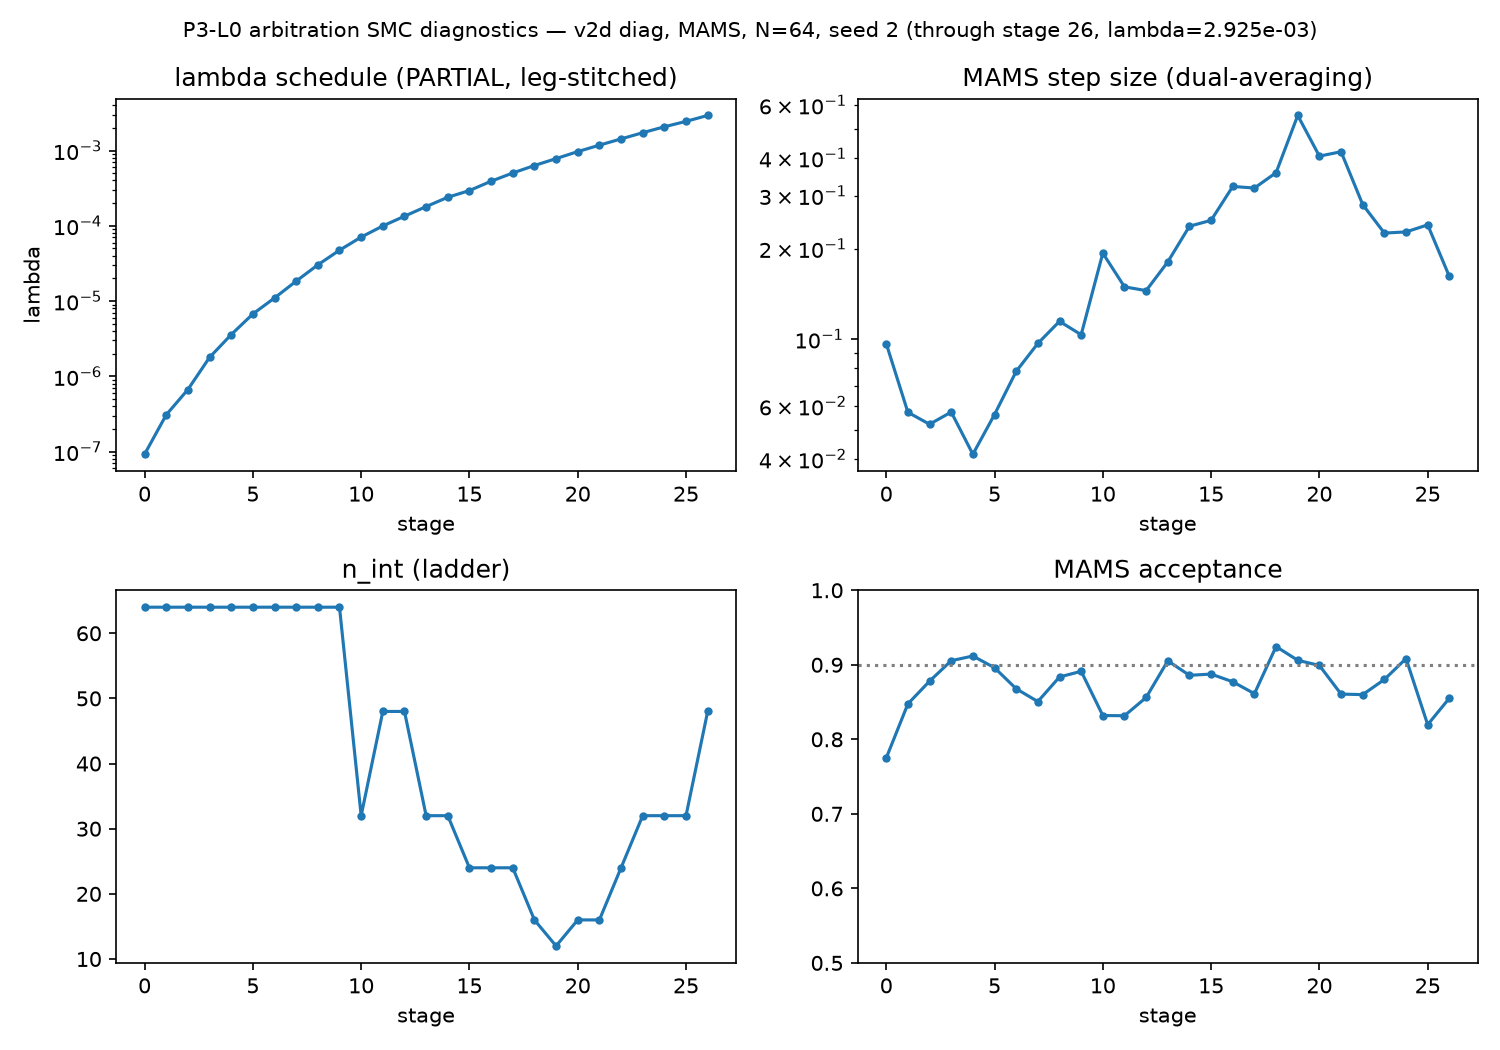
\includegraphics[width=0.72\textwidth]{../figs/l0_smc_traces_partial.png}
\caption{The arbitration MC-SMC arm on the 46-d cond-$10^{14}$
\dfile{v2d} target (job 56168446): healthy per-stage diagnostics to
$\lambda=0.587$ at the 3.5-h A100 fence --- budget-infeasible, not
unhealthy. Together with the L4 resume leg ($\lambda=0.4183$ at a 12.26-h
leg, on-disk record) and the classic arm's NO-VERDICT, this is the
vehicle-exhaustion evidence behind the anchor arbitration's
PARTIAL-BY-VEHICLE-EXHAUSTION close. Disposition:
\dfile{research/gate\_ledger\_final.md}.}
\label{fig:l0traces}
\end{figure}

\subsection{Easy scene (B3): double-blocked, and honest about it}
\label{sec:matrix:b3}

The nominally easiest row --- four 22-d unimodal systems from the
hundred-systems class --- returned no evaluable accuracy cell, for two
independent reasons that we report as such. The SMC arms are
{\bf blocked by budget}: no arm finished inside the pre-registered 5-h/arm
free-tier L4 fence at $N{=}512$ (12.38 L4 GPU-h consumed; the readable
result is the cost row: scene-substrate MC-SMC at $N{=}512$ costs
$>5$\,h/target on an L4).\art{data/b3\_cells.json} The classic reference
arms are {\bf blocked by reference}: all four posteriors completed but all
four fail the frozen reference-acceptance rule
($\Rhat_{\rm worst}$ 4.36--7.87 vs.\ $<1.05$; $\ESS_{\min}$ 63.7--84 vs.\
$\ge200$), so ``4/4 references complete'' must not be read as ``references
usable'' --- each per-cell artifact records
\texttt{reference\_accepted:\,false}. The double block is itself a datum:
it is additional, independent evidence for the single-stage-recipe
convergence finding above, on targets designed to be easy.

\begin{figure}[htbp]
\centering
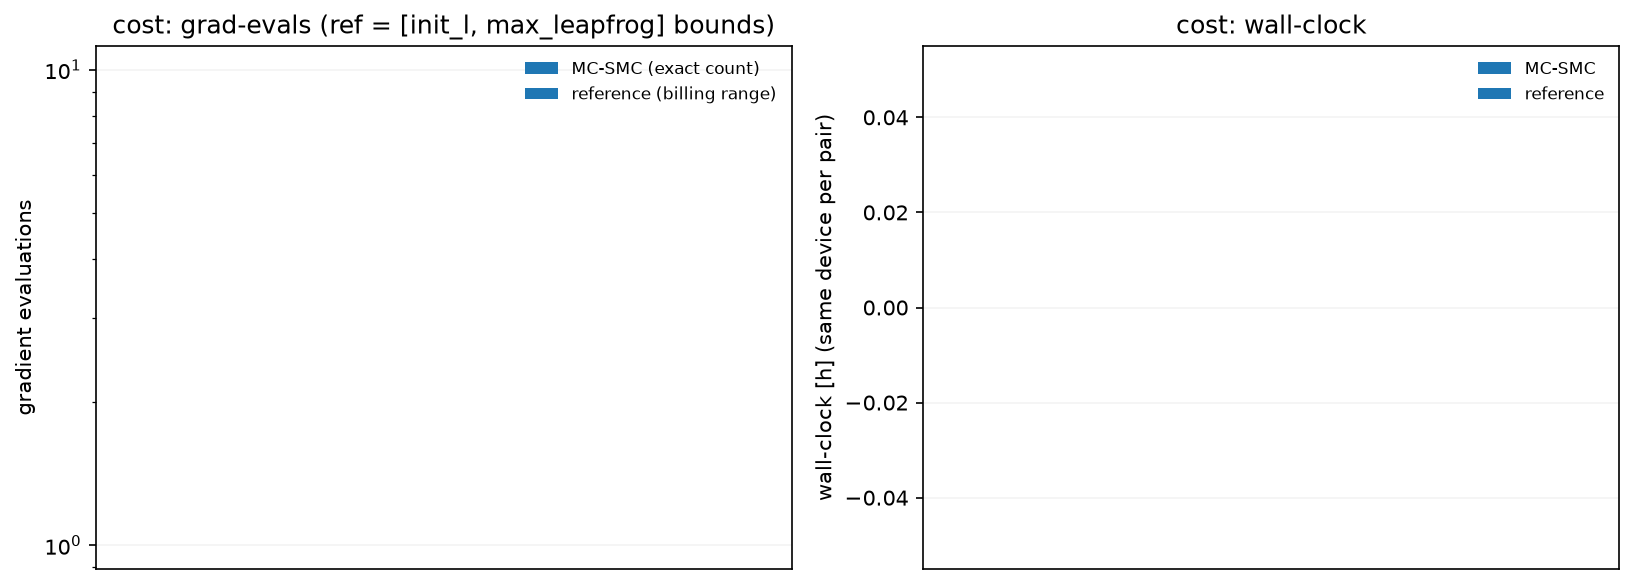
\includegraphics[width=0.8\textwidth]{../figs/b3_cost.png}
\caption{B3's readable result is its cost row: scene-substrate MC-SMC at
$N{=}512$ costs $>5$\,h per 22-d target on the free-tier L4 (12.38 L4
GPU-h consumed, 0/4 arms complete inside the pre-registered 5-h/arm
fence). Source: \dfile{data/b3\_cells.json}.}
\label{fig:b3cost}
\end{figure}

\subsection{Two cross-cutting findings}
\label{sec:matrix:crosscutting}

{\bf (A) Bootstrap error bars understate evidence error.} Measured twice,
in different ways. At B0, MAMS-SMC on the analytic ill-conditioned target
returns \logZ\ $-145.80$ vs.\ the analytic $-148.20$: a 2.40-nat error at
$\sboot=0.37$, i.e.\ $6.6\sboot$ (the HMC-mutation arm errs by 21.6 nats at
$\sboot=0.41$).\art{data/smc\_b0\_report.json} On DSPL, on {\it identical
data} where an exact reparameterization forces the true difference to zero,
$\dlogZ(\mathrm{orig}-\mathrm{ratio})=+3.06\pm0.35_{\rm boot}$. The
practical rule the campaign adopted, and that we recommend: never gate a
\dlogZ\ claim on \sboot\ alone; the seed-repeat scale ($\sseed=1.79$ nats
here, $n{=}3$, $\pm46\%$ sampling error on that estimate) is the
load-bearing error bar for every evidence gate.

{\bf (B) Frozen-reference coverage risk.} The B5-G2 fail decomposes into
both-basin positive evidence offsets with both ensembles
$\gammaEPL$-disjoint from the reference chains and two independent kernels
agreeing on the new location (\S\ref{sec:matrix:b5}): frozen references
built from short fixed-step MCMC chains can carry within-basin coverage
error far exceeding the $\sigma$-scale of any gate built on them. The X2
frozen-set validity question (\S\ref{sec:gifts:x2}) is the same genus on
the SBC side. The lesson we apply to ourselves first: an evidence reference
needs a coverage certificate before it is frozen into a gate.

Finally, the demotion that held all campaign: {\bf unadjusted-MCLMC
mutations are not an evidence kernel}. The B0 bias screen measured
$\dlogZ=+10.79\pm0.54$ vs.\ MAMS on the ill-conditioned target ---
$20.1\sigma$ by the artifact of record (the ledger prose says ``$30\sigma$'';
the flagged, binding artifact value is
$20.1$)\art{data/smc\_b0\_report.json} --- and B5-G3's $\times56$
minor-mode inflation confirms the channel on a real-lens-derived target.
Within-basin locations stay correct in both measurements: MCLMC remains
useful precisely as the cheap {\it diagnostic} it was demoted to.

%%%%%%%%%%%%%%%%%%%%%%%%%%%%%%%%%%%%%%%%%%%%%%%%%%%%%%%%%%%%%%%%%%%%%%%%%%%%%%%
\section{Calibration Gifts and the Handoff Package}
\label{sec:gifts}
%%%%%%%%%%%%%%%%%%%%%%%%%%%%%%%%%%%%%%%%%%%%%%%%%%%%%%%%%%%%%%%%%%%%%%%%%%%%%%%

\subsection{X2: the first formal SBC of the pipeline class}
\label{sec:gifts:x2}

The X2 cross-pollination arm ran the first formal simulation-based
calibration (SBC; rank-statistic) test of this pipeline class: $N{=}32$
prior-matched mock systems through the certified port of the classic
MAP$\to$SVI$\to$HMC pipeline at reduced free-tier budgets ($\sim$29 A16-h;
$N{=}32$ of the assigned $\ge64$ --- an under-delivery selected by the
pre-stated budget rule and reported as such). Every verdict is
{\it proposed (UNCERTIFIED --- external)}: the ranks are the deliverable;
interpretation and certification belong to the team.\art{data/x2\_sbc.json}

Three results, in decreasing order of confidence. {\bf (i) A validity
question about the frozen mock set}, posed as a question and not a finding
of fault: the pre-existing frozen SBC set carries, per its own provenance
in the upstream development branches, a generation prior narrower than the
current fitting prior --- under which SBC fails by construction (truth
draws must follow the fitting prior). Such a mismatch is a legitimate
robustness-testing design if intentional; the question for the team is
whether a matched-prior set should exist. Our arm therefore ran on
prior-matched {\it regenerated} mocks. (Detail is internal-memo material,
publication-gated on the team's sign-off.) {\bf (ii) Severe lens-light rank
miscalibration}: the lens-light photometric block shows one-sided,
sign-coherent rank pile-ups --- $I_e$ rank-location $z=-5.27$
($p=7.6\times10^{-11}$; 18/32 systems in the bottom bin), $R_{\rm s\acute ersic}$
$z=+5.76$ ($p=1.5\times10^{-10}$), $n_{\rm s\acute ersic}$ $z=+4.75$ ---
which is not an under-mixing shape; three candidate channels (genuine
pipeline miscalibration, reduced MAP/SVI budget, plug-in error map) are not
separable from this run and are said so in the claims register. The mass
block shows no location bias (worst $|z|=2.25$) but 6 of 8 parameters fail
uniformity via U-shapes, the classic under-mixing signature, with only 2 of
32 fits passing the health rule at this budget. {\bf (iii) The glass-house
disclosure}, included in the same harness by pre-registered rule: our own
previous campaign's E1c SBC {\it failed} the same $\gammaEPL$-rank gate
($p=6.5\times10^{-5}$, 68\% coverage 0.34) and {\it flipped to PASS}
($p=0.53$) when unhealthy fits were rerun deep and re-read healthy-only ---
sampler pathology can fake rank failures, and that amendment path is
exactly what $n_{\rm healthy}=2$ blocks here. The turnkey harness ships in
the handoff package for an $N\ge64$ rerun at reference
settings.\art{research/x2\_sbc\_gift.md}

\begin{figure}[htbp]
\centering
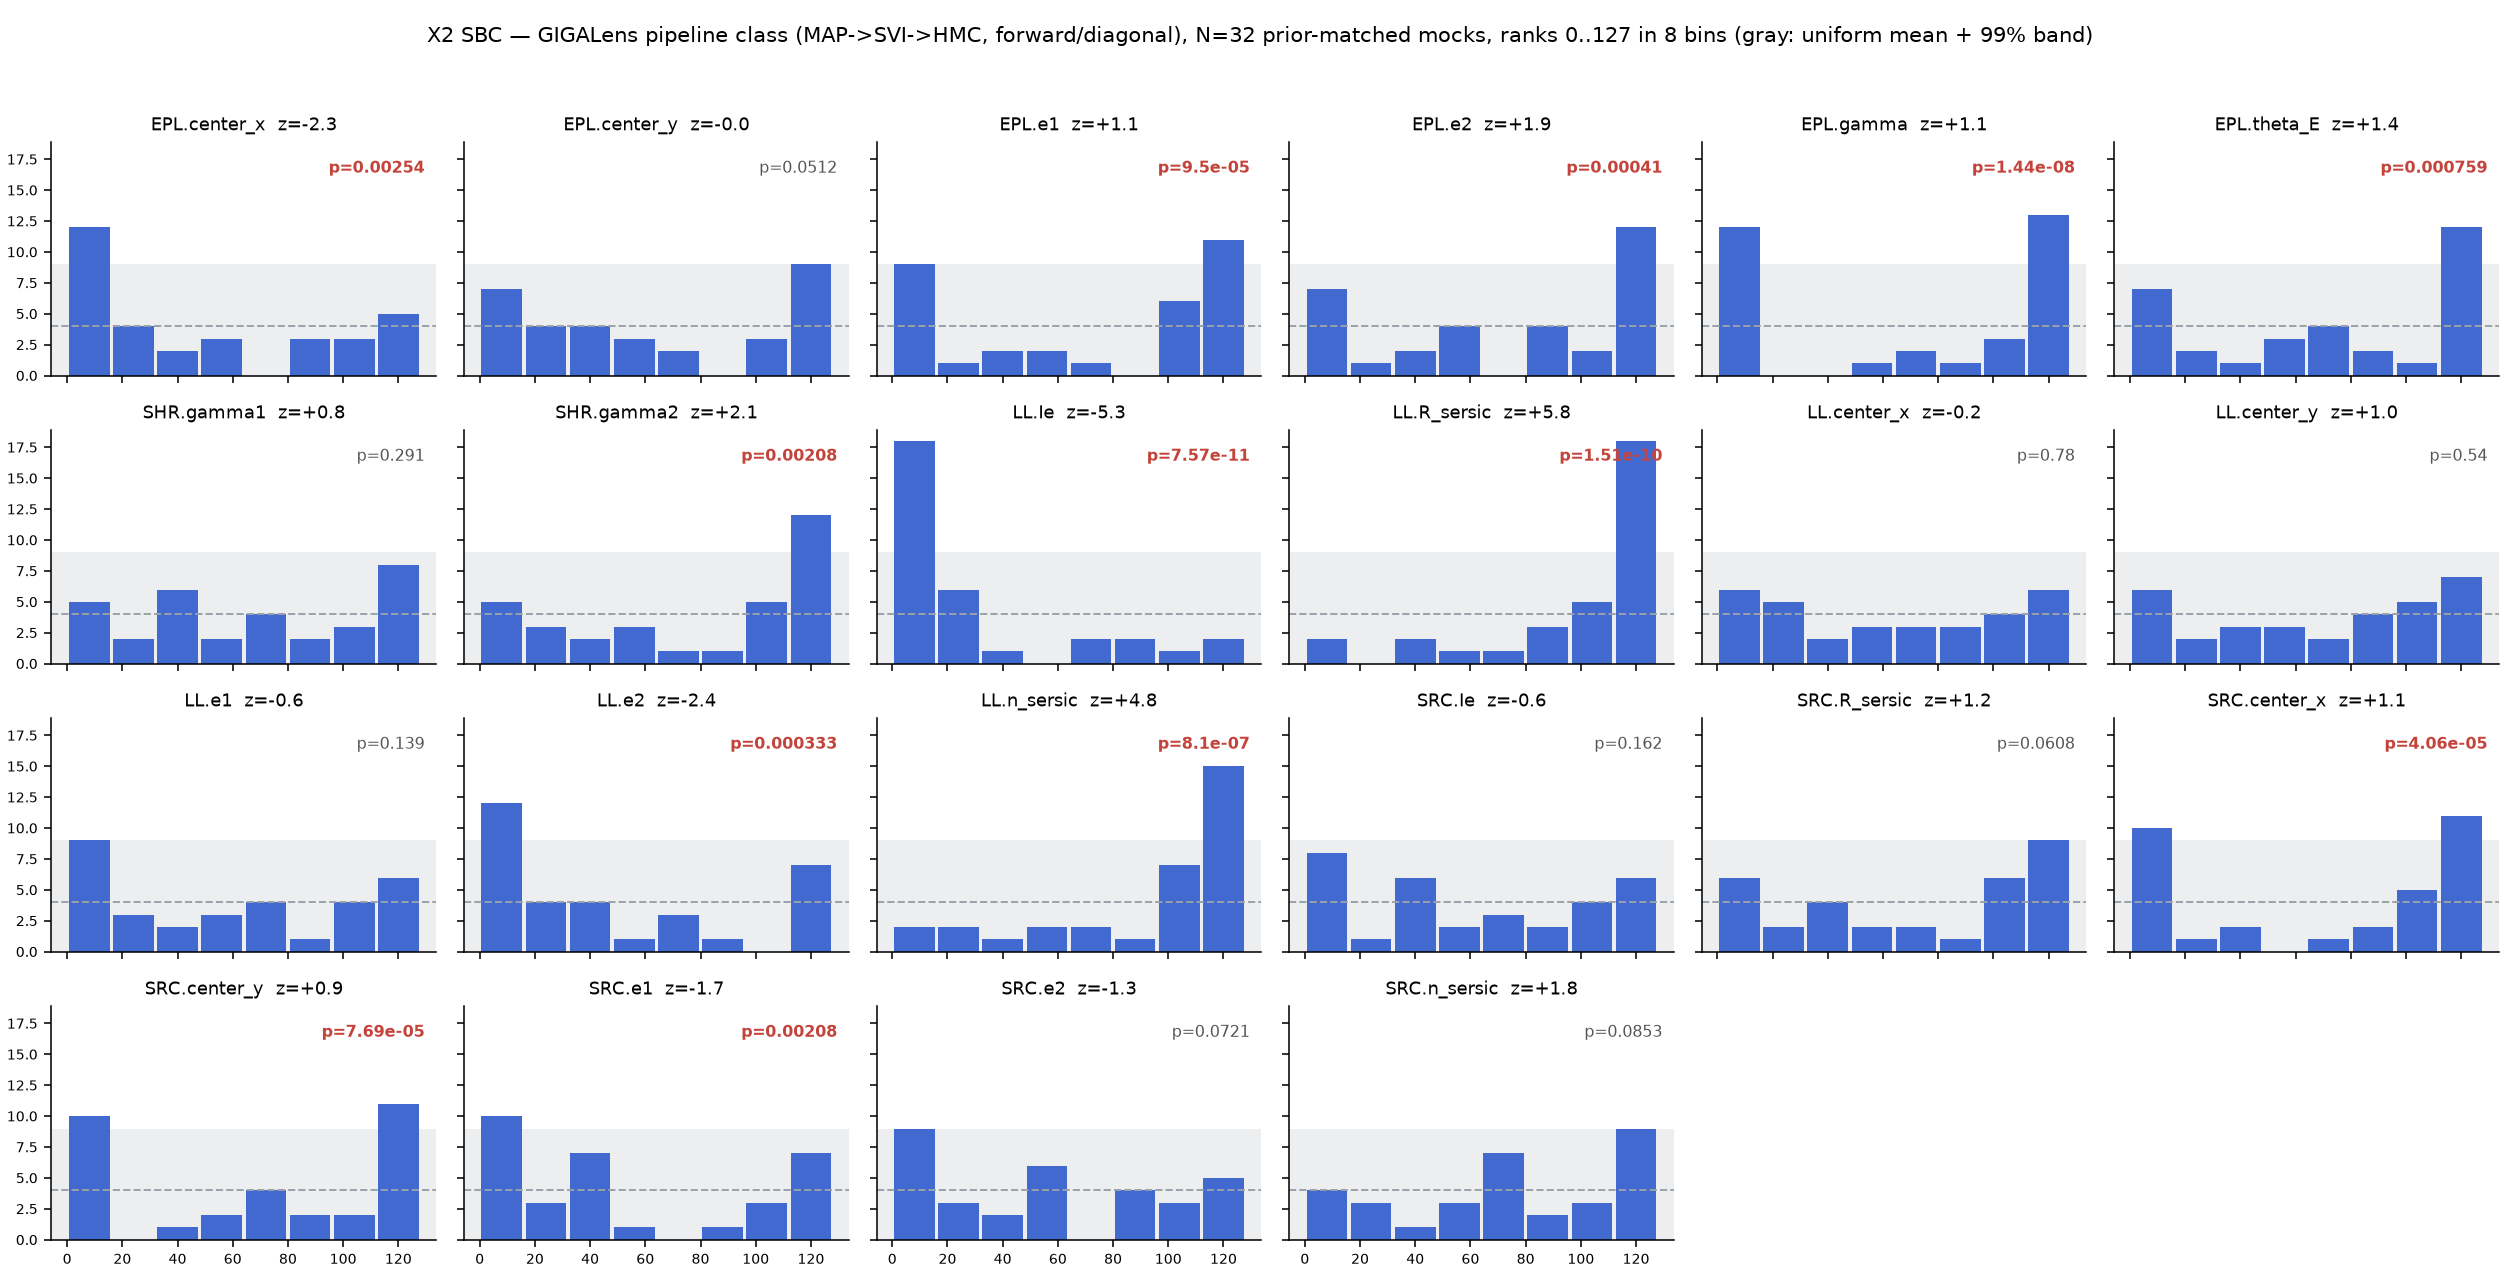
\includegraphics[width=0.95\textwidth]{../figs/x2_rank_hist_grid.png}\\[4pt]
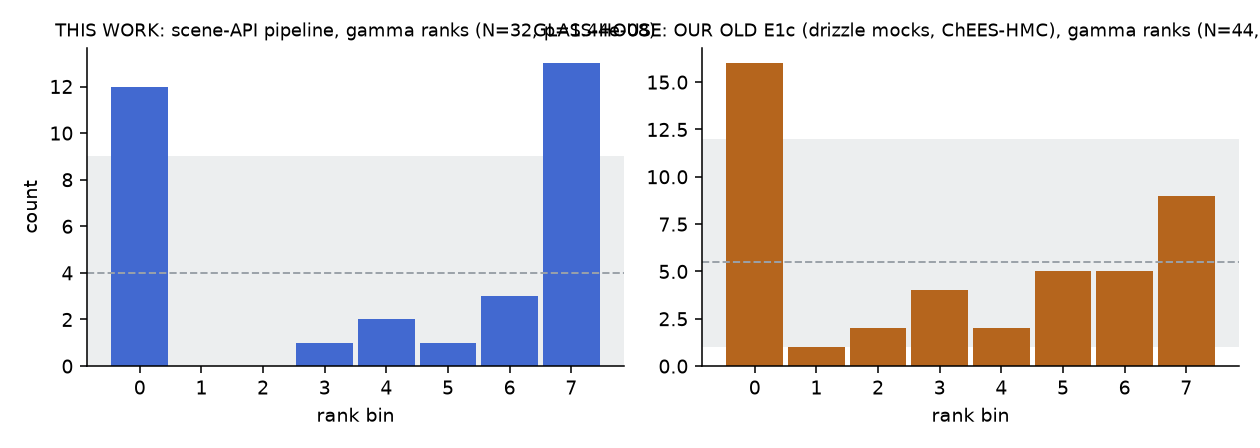
\includegraphics[width=0.62\textwidth]{../figs/x2_rank_hist_glasshouse_gamma.png}
\caption{X2: the first formal SBC of the pipeline class ($N{=}32$
prior-matched mocks, reduced free-tier budget; all verdicts proposed,
UNCERTIFIED --- external; the pipeline runs on the upstream development
branches, whose unpublished results are not characterized here). Top:
rank histograms --- the lens-light photometric block shows one-sided,
sign-coherent pile-ups ($|z|$ up to 5.76), which is not an under-mixing
shape; the mass block shows under-mixing U-shapes without location bias
(worst $|z|=2.25$). Bottom: the glass-house disclosure --- our own
previous campaign's E1c $\gammaEPL$-rank gate failed
($p=6.5\times10^{-5}$) and flipped to PASS ($p=0.53$) when unhealthy
fits were rerun deep and re-read healthy-only: sampler pathology can
fake rank failures, and $n_{\rm healthy}=2$ blocks that amendment path
here. Source: \dfile{data/x2\_sbc.json}.}
\label{fig:x2}
\end{figure}

\subsection{The handoff package}
\label{sec:gifts:handoff}

The handoff directory (\dfile{papers/handoff/}) contains the engagement
memo (with its close-of-campaign addendum) and \dfile{CLAIMS.md}: fourteen
claims in the receiving team's own claims-register format, every verdict
{\it proposed (UNCERTIFIED --- external)}, with the sign-off-gated claims
(those touching data or targets from the upstream development branches)
explicitly marked, and a mandatory doubt report attached to each. That file
--- not this report --- is the interface of record for the team: it names
the artifact behind every number and reserves ``validated'' for the old
certified stack throughout.

The gap list \dfile{research/handoff\_gap\_list.md} inventories the
package honestly against what the plan promised: delivered in substance are the
claims register, the certified correlated-noise likelihood port
(\dfile{cgl2/correlated.py}, \dfile{cgl2/marg.py}, with its exact-limit
validation record), the tempered-SMC implementation with
checkpoint/resume (\dfile{cgl2/samplers/}, 58-test suite), and the turnkey
SBC harness (\dfile{30\_sbc\_gift.py}). Promised but {\it not} packaged at
close: the SMC-stage adapter specification, the correlated-likelihood
handoff document and upstream-shaped patch files, the DSPL note, and the
Hessian-stage restore (never started). These remain owed offers, listed as
such in the memo addendum, not silently dropped.

%%%%%%%%%%%%%%%%%%%%%%%%%%%%%%%%%%%%%%%%%%%%%%%%%%%%%%%%%%%%%%%%%%%%%%%%%%%%%%%
\section{Discussion}
\label{sec:discussion}
%%%%%%%%%%%%%%%%%%%%%%%%%%%%%%%%%%%%%%%%%%%%%%%%%%%%%%%%%%%%%%%%%%%%%%%%%%%%%%%

\subsection{What the campaign settles}

Five things are now measured that were conjectures at the start. (1) {\bf
The bridge holds}: the scene-substrate forward model is certified against
the validated old stack at machine precision for our config class, and the
correlated-noise likelihood ported onto it reproduces the certified
real-lens result on an independent stack and machine ---
$\gammaEPL$ to $\Delta=0.0027$ and \logZ\ to 0.11 nats (L0-G2). The
$\gammaEPL=1.103$ result now stands on two stacks. (2) {\bf The mechanism
narrows}: stationarity of the noise-model class behind that number is
rejected on the real field ($p=0.010$, replicated spatial pattern), the
companion and spectrum-flooring suspects are eliminated, and the
profile-curvature fork died at its zero-cost entry gate --- noise-model
{\it class} misspecification is the standing working hypothesis for the
over-correction, with source/PSF representation the surviving alternative.
(3) {\bf \mcsmc\ is the campaign's only evidence-producing vehicle}, and
its failure mode is purely economic: cost walls on healthy samplers, never
divergence or mode loss. (4) {\bf Unadjusted MCLMC is not an evidence
kernel} ($20.1\sigma$ screen; $\times56$ minor-mode inflation;
locations intact) --- but is a cheap, useful diagnostic. (5) {\bf The
classic single-stage recipe does not converge on this posterior family},
now shown on both stacks and three independent cells (B3, arbitration, X2
health rates); the two-stage re-preconditioned recipe remains the only
known converging direct-sampler path.

A post-campaign epilogue (E1, 2026-07-22; PI-requested MCLMC fits of both
diagonal targets, \S\ref{sec:modelers}) sharpened two of these after
close. On (5), the direct-sampler gap is narrower than the campaign body
suggests: the team's own vendored MCLMC, warm-started and run with its
windowed mass-matrix adaptation and regularization option, delivered the
first fully convergence-certified posterior on the \dfile{v2d} native
diagonal target ($\Rhat_{\rm worst}=1.0031$, $\ESS_{\min}=30{,}334$;
$\gammaEPL=1.4683\,[1.4343,1.5048]$, $0.72\sigma_{\rm comb}$ from the
anchor) at 1.49 free-tier L4-hours --- so the convergence failures above
are specific to the classic single-stage recipe, not to direct samplers
per se. On (2), the mechanism gains its sampling-side face: on the binned
product the same vehicle under the same \emph{diagonal} likelihood
migrated every one of 64 chains, in all four seed groups, out of the
physical basin it was warm-started in and down to
$\gammaEPL\approx1.08$--$1.15$ (kept-draw pooled median 1.1047, 0.0015
from the correlated fit's 1.1032; NO-QUOTE --- the ensemble fails every
gate, and the one allowed escalation was declined because migration is
structural, not a depth problem). The binned data's preference for the
unphysical low-$\gammaEPL$ shelf is therefore a property of the
\emph{product}, not of any single likelihood or sampler: it is reached by
tempered SMC under the correlated likelihood and, from a physical-basin
warm start, by MCLMC under the plain diagonal one --- which is the T0.4 mechanism
narrative restated from the sampling side, and one more reason the
mechanism's confirmatory data-side injection test (above) is worth
running.\art{data/e1\_harvest.json}

%%%%%%%%%%%%%%%%%%%%%%%%%%%%%%%%%%%%%%%%%%%%%%%%%%%%%%%%%%%%%%%%%%%%%%%%%%%%%%%
%% E2 epilogue subsection (2026-07-23, second post-campaign epilogue).
%% Every number traces to data/e2_harvest.json, data/mclmc_diag_odell.json,
%% data/o4_{v3b,v2d}_stage2.json, data/odell_registration.json (via the
%% packaged data/odell_cutout.npz meta), and data/e2_odell_noise.json; the
%% pre-registered records are the CAMPAIGN.md E2 design checkpoint and
%% research/checkpoint_e2_o4.md (both frozen before any GPU work).  Bright
%% lines: NO gamma quoted from a failed fit (telemetry/descriptive labels
%% throughout); O4 is framed as a service finding and, like the rest of the
%% epilogue's collaborator-facing wording, ships through the PI's review
%% before anything external (SIGNOFF_CHECKLIST discipline).
%%%%%%%%%%%%%%%%%%%%%%%%%%%%%%%%%%%%%%%%%%%%%%%%%%%%%%%%%%%%%%%%%%%%%%%%%%%%%%%
\subsection{Epilogue E2: the collaborator's own data --- registration, the
apples-to-apples fit, and two service findings}
\label{sec:e2}

After E1, a collaborator on the team's sampling effort (E.~Odell) shared
his own working cutout and PSF of \foundry\ --- $140^2$ cutout, $29^2$
PSF, with no error map, mask, pixel scale, or exposure metadata attached
--- together with a workflow report (priv.\ comm.): his own first-stage
MCLMC had ``very migratory chains,'' and a second stage preconditioned on
the first stage's tail converged $\Rhat\ll1.01$ at $\sim$8--16 chains
$\times$ $\sim$5000{+}5000 draws. E2 is the pre-registered epilogue on
that material: registration and packaging (O1), the apples-to-apples
MCLMC fit under the E1-frozen gates (O2), a noise audit of his
preparation with the T0.4-1 machinery (O3), and a demonstration of his
stage-2 rescue on our own stored E1 chains (O4, run on \emph{our} data
only). All gates were frozen before any GPU work; everything ran on the
free tier (6.8 L4-h total; no A100-h), and his data stays outside the
repository per the campaign's data bright line.\art{data/e2\_harvest.json;
CAMPAIGN.md E2 design checkpoint; research/checkpoint\_e2\_o4.md}

\paragraph{Registration (O1): a fourth pixelization, a parity flip, and a
stack-dependent companion.}
Registered against our calibrated $0.04''$ fine product
(arcsinh-stretched, high-pass-filtered ZNCC over a scale grid and all
eight dihedral orientations), his cutout sits at $0.064125''$/px ---
\emph{exactly half our native $0.12825''$}, a fourth pixelization of this
sky beyond our $0.128''/0.08''/0.04''$ trio, and measurably \emph{not}
the $0.065''$ paper-drizzle scale --- with a \emph{parity flip} (a
left-right mirror) relative to our raster; registration residual
$0.300$\,px against a $0.5$\,px gate. His PSF is sampled at the cutout's
own scale (decisive: the half-scale hypothesis drops the aligned cosine
from $0.885$ to $0.705$) and is \emph{sharper and more symmetric} than
our empirical PSF (moment-FWHM $0.449''\times0.456''$ vs.\
$0.555''\times0.475''$). Two preparation-level findings fell out of the
registration census. First, the bright compact companion at
$(-2.34'',-2.86'')$ --- masked by our pipeline and a named suspect
earlier in the campaign (T0.3, \S\ref{sec:modelers} item~2 sources) ---
\emph{exists only in our stack}: his frame shows nothing at that
position, while carrying nine compact sources ours lacks
(single-visit-class artifacts; all masked) --- a drizzle
epoch/frame-selection question for the collaborator, not a science claim.
Second, his files carry no noise model, so the packaged error map is a
\emph{documented v1 assumption} (background RMS from his own empty sky
plus our archival exposure metadata; packaged sky
$\chi^2/\mathrm{px}=0.9987$), to be replaced by his exact numbers.%
\art{data/odell\_registration.json; data/odell\_cutout.npz (meta)}

\paragraph{The apples-to-apples fit (O2): pre-registered fork 2 fires.}
The E1 vehicle --- constants, warm-start path, and both frozen gates
byte-identical; the registered flip and offset absorbed grid-side so
priors and warm starts remain in the campaign frame --- was warm-started
from the transported healthy anchor cloud (median $1.4334$). Every one of
the 64 chains in all four seed groups migrated during the 2000-step
burn-in to the same low-$\gammaEPL$ shelf (Fig.~\ref{fig:e2migration}):
kept-draw pooled median $1.0999\,[1.0727,1.1103]$ --- \emph{descriptive
telemetry, not a quotable posterior}: the fit fails both frozen gates
($\Rhat_{\rm worst}=5.46$, $\ESS_{\min}=66$; all 64 chains spend
\emph{every} kept draw outside the $[1.15,2.0]$ band), and the one
allowed escalation was declined for the E1 reason (structural migration,
not sampling depth). Per-chain migration $\Delta\gammaEPL=0.27$--$0.45$;
the endpoint sits $0.0033$ from the certified corr-low $1.1032$ and
$0.0048$ from the E1 \dfile{v3b} shelf. Of the three pre-registered
interpretation forks, fork~1 --- the native answer robust across four
pixelizations, the strongest closure available --- is dead for the
resampled family; \textbf{fork~2 fires}: the migration extends to a
second resampled product \emph{and} a second, fully independent
preparation pipeline, on the collaborator's own data --- matching his
independent ``very migratory chains'' report, so the pathology is not an
artifact of our preparation. A goodness-of-fit finding rode along: even
the fit's best kept draw leaves $\chi^2/\mathrm{px}=26.8$ under the v1
noise model (the shelf fit is a grossly bad model of his data, not merely
an unconverged one), and the pooled per-dimension median is off-manifold
at $\chi^2/\mathrm{px}=72.7$ --- medians of unconverged multi-basin
ensembles are not models.\art{data/mclmc\_diag\_odell.\{npz,json\};
data/e2\_harvest.json; data/e2\_odell\_noise.json (model\_render)}

\begin{figure}[htbp]
\centering
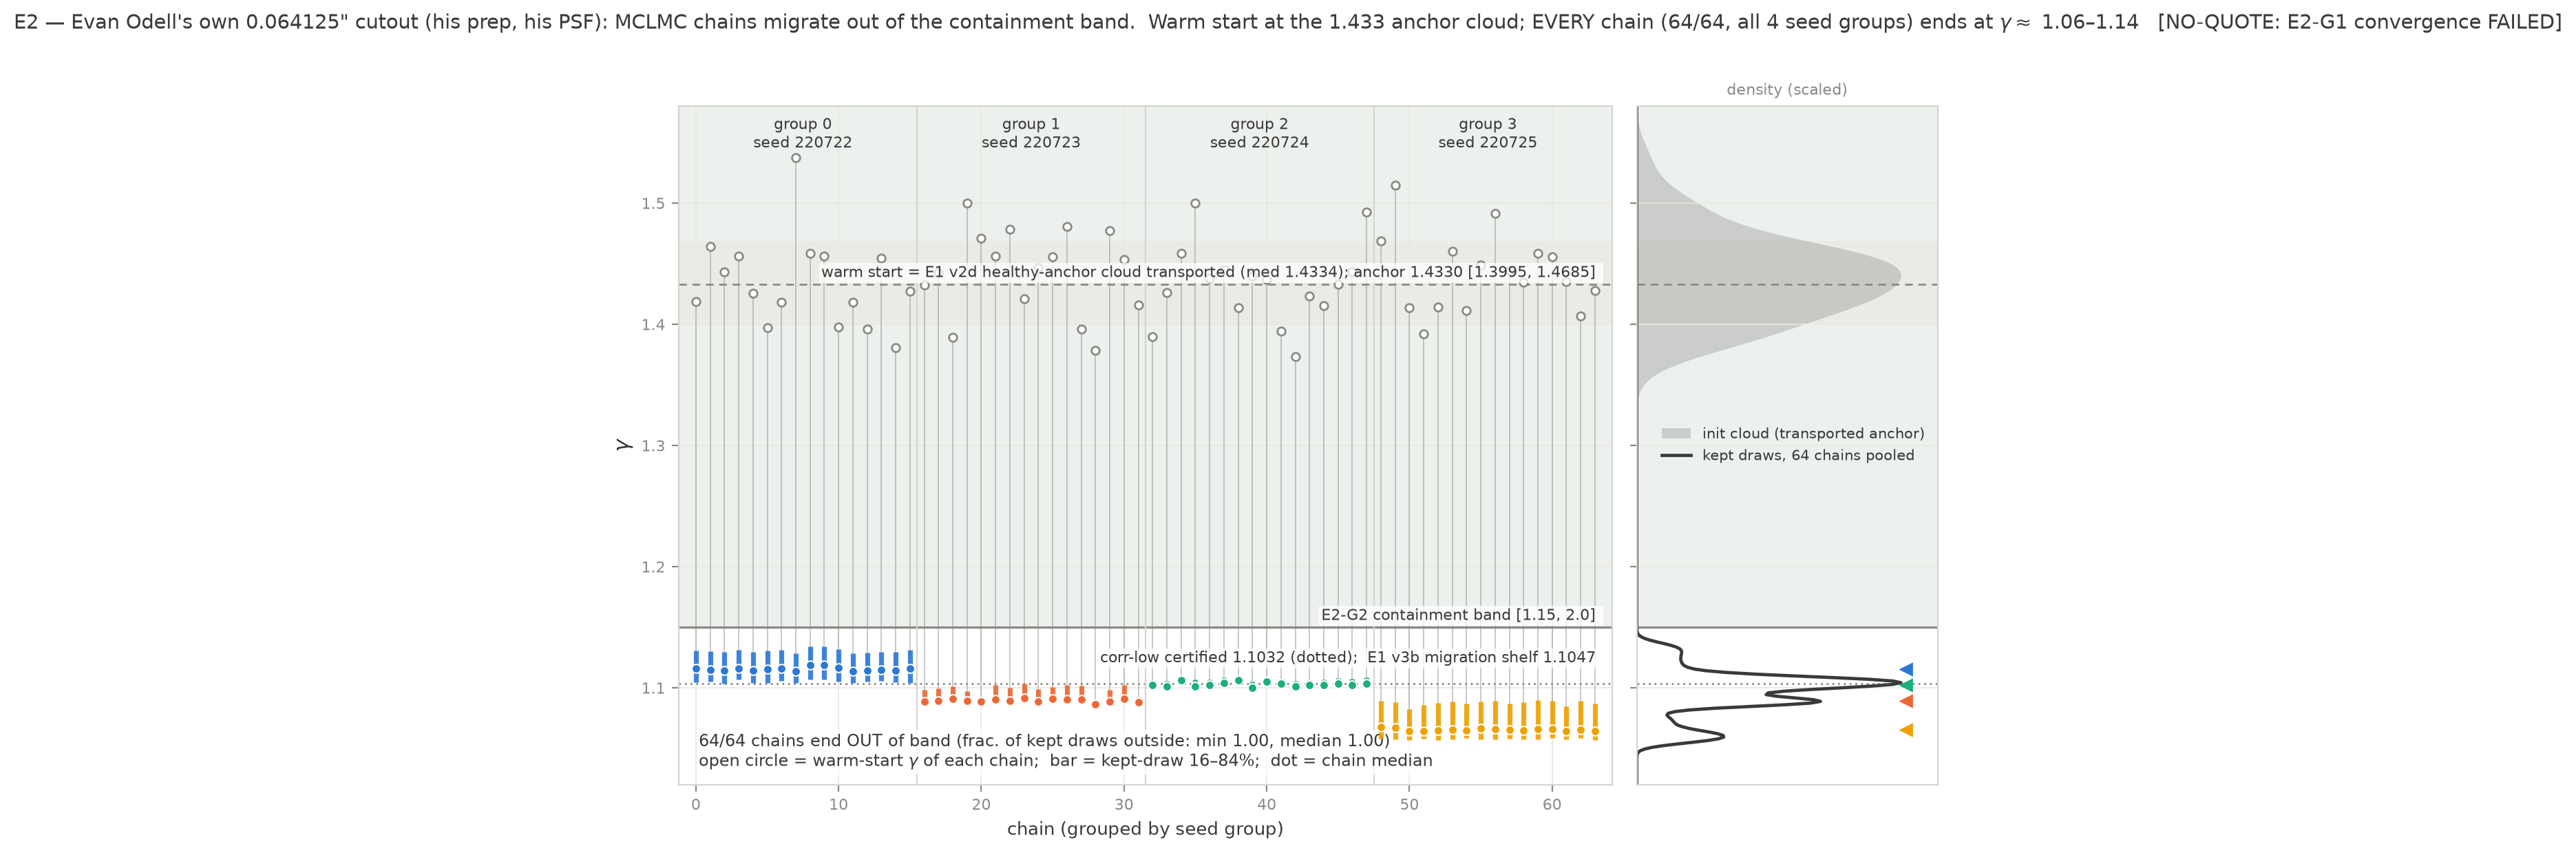
\includegraphics[width=0.98\textwidth]{../figs/e2_odell_migration.png}
\caption{The E2 apples-to-apples fit on the collaborator's own registered
$0.064125''$ product (his preparation, his PSF; plotted before gate
math). Left: for each of the 64 chains (colored by seed group), the
warm-start $\gammaEPL$ (open circle, drawn from the transported healthy
$1.433$ anchor cloud) against its kept-draw 16--84\% interval and median:
every chain exits the E2-G2 containment band $[1.15,2.0]$ during burn-in
and equilibrates at $\gammaEPL\approx1.06$--$1.14$ (fraction of kept
draws outside the band: min 1.00, median 1.00 --- every kept draw; all 64
violations reported, none dropped). Right: init-cloud vs.\ pooled
kept-draw marginals; the pooled kept-draw median 1.0999 sits 0.0033 from
the corr-low certified 1.1032 and 0.0048 from the E1 \dfile{v3b}
migration shelf 1.1047 --- descriptive only (the ensemble fails both
frozen gates, $\Rhat_{\rm worst}=5.46$, NO-QUOTE). Source artifacts:
\dfile{data/mclmc\_diag\_odell.\{npz,json\}}
(\texttt{gates.E1\_G2.violations});
\dfile{data/e2\_harvest.json}.}
\label{fig:e2migration}
\end{figure}

\paragraph{The stage-2 rescue demonstration (O4): falsifier fired,
control held.}
This experiment ran entirely on our own stored E1 chains, and is offered
as a service finding about the shared two-stage recipe (the
collaborator's rescue is empirically the same move as the two-stage
re-preconditioned recipe used throughout this program --- ours included).
The pre-registered prediction: a stage-2 MCLMC preconditioned on the
migrated \dfile{v3b} stage-1 tail (init draws, tail covariance as inverse
mass, tail mean; 16 chains $\times$ 5000{+}5000 at the collaborator's
stated scale) would converge pristinely \emph{at} the shelf ---
demonstrating that stage-2 convergence metrics cannot detect stage-1
basin selection. \textbf{The falsifier fired instead}, and per the frozen
checkpoint it is reported as loudly as a pass: stage-2
$\Rhat_{\rm worst}=1.1875$, $\ESS_{\min}=81$ ($\Rhat_\gamma$ 1.128) ---
no pristine-$\Rhat$-at-the-shelf at these settings. What survives is a
weaker but still useful statement (Fig.~\ref{fig:e2rescue}): the rescue
moves the diagnostics most of the way toward the pass region
($\Rhat_{\rm worst}$ $1.379\to1.188$, $\Rhat_\gamma$ $1.261\to1.128$)
while the chains stay at the shelf ($\gammaEPL$ median 1.0849, telemetry;
$-0.019$ vs.\ the stage-1 tail --- falsifier F2, a return toward the
band, did \emph{not} fire, so the E1/E2 migration interpretation stands);
a looser-but-common threshold ($\Rhat<1.2$) \emph{would} have certified
the unphysical solution, and the split-half readout ($\Rhat_{\rm worst}$
1.033 on chains 0--7 vs.\ 1.321 on 8--15) shows an 8-chain practitioner
could land on either side --- at the rigorous frozen gates
($\Rhat<1.01$, $\ESS\ge1000$) the diagnostics still flag stage-1 basin
selection. The control held exactly as pre-registered: the identical
rescue on the healthy \dfile{v2d} stage-1 converges cleanly at the E1
posterior ($\Rhat_{\rm worst}=1.0029$, $\ESS_{\min}=8305$;
$\gammaEPL=1.4683$, $0.0008\sigma_{\rm comb}$ from the E1 quotable value;
0/16 chains out of band) --- the property probed is stage-1-conditional,
as designed. The collaborator's reported $\Rhat\ll1.01$ second stage is
\emph{not} reproduced on our stored chains at his stated scale;
understanding that difference needs his exact configuration (chain count
and length, preconditioning details, thresholds) --- a question for him,
not an assumption in this report.%
\art{data/o4\_\{v3b,v2d\}\_stage2.\{npz,json\};
research/checkpoint\_e2\_o4.md; data/e2\_harvest.json}

\begin{figure}[htbp]
\centering
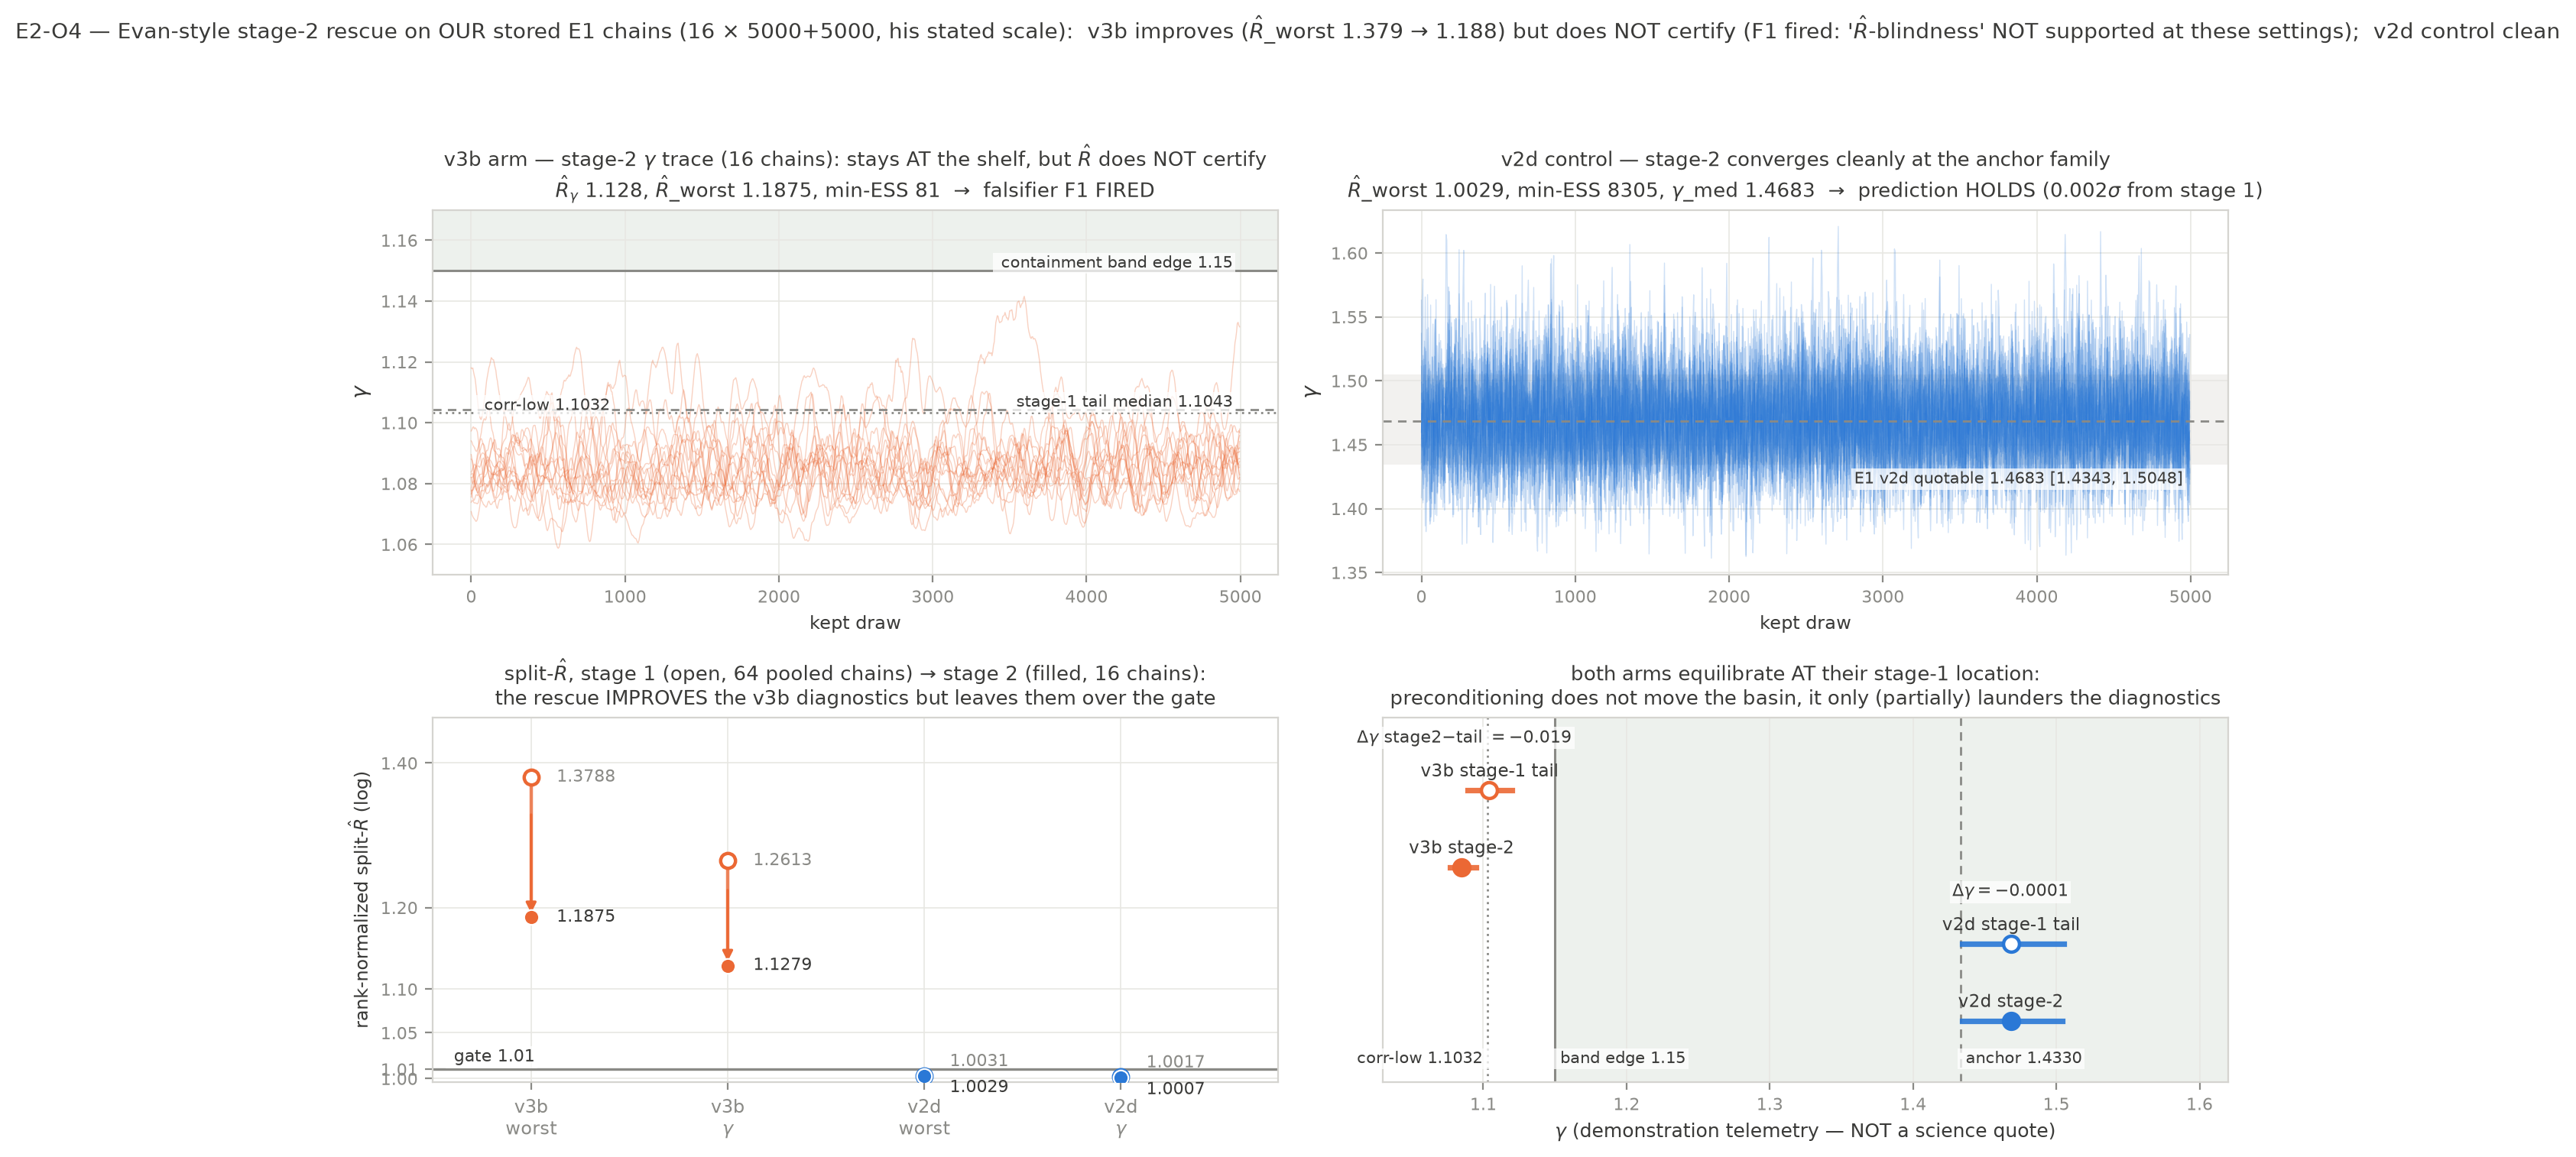
\includegraphics[width=0.98\textwidth]{../figs/e2_o4_rescue.png}
\caption{The O4 stage-2 rescue demonstration on our stored E1 chains
(16 $\times$ 5000{+}5000, the collaborator's stated scale; plotted before
gate math). Top left: the \dfile{v3b} arm's stage-2 $\gammaEPL$ trace
stays at the migrated shelf but does not certify ($\Rhat_\gamma$ 1.128,
$\Rhat_{\rm worst}$ 1.1875, min-\ESS\ 81 --- falsifier F1 fired). Top
right: the \dfile{v2d} control converges cleanly at the anchor family
($\Rhat_{\rm worst}$ 1.0029, min-\ESS\ 8305), matching the E1 quotable
posterior to $0.0008\sigma_{\rm comb}$. Bottom left: stage-1 (open)
$\to$ stage-2 (filled) split-$\Rhat$ dumbbells against the 1.01 gate ---
the rescue improves the \dfile{v3b} diagnostics but leaves them over the
gate. Bottom right: both arms equilibrate \emph{at} their stage-1
location (all $\gammaEPL$ values demonstration telemetry, not science
quotes): preconditioning does not move the basin. Source artifacts:
\dfile{data/o4\_\{v3b,v2d\}\_stage2.\{npz,json\}};
\dfile{research/checkpoint\_e2\_o4.md}; \dfile{data/e2\_harvest.json}.}
\label{fig:e2rescue}
\end{figure}

\paragraph{The noise audit (O3): his preparation is correlated like ours;
the stationarity verdict is model-quality-limited.}
The T0.4-1 machinery (masked ACF, two-component drizzle-family fit,
$3\times3$ block stationarity against a 200-draw calibrated null) was run
on his product in two arms --- the pre-declared model-subtracted arm
(residuals of the best available model on his grid: the failed fit's
maximum-log-density kept draw, a residual-minimizing reference point, not
a certified posterior) and a no-model robustness arm added because that
model is poor; only verdicts on which \emph{both} arms agree are claimed.
\textbf{Correlated like ours --- confirmed on both arms}
(Fig.~\ref{fig:e2noise}): nearest-lag $\rho_{01}/\rho_{10}$ =
$0.844/0.807$ (no-model) and $0.762/0.847$ (model-subtracted) against the
pure-drizzle prediction $0.600$ at his scale ratio --- excess correlation
\emph{above} the entire drizzle-registration envelope $[0.51,0.66]$ ---
with the same drizzle$+$background kernel family as our products (fitted
correlated weight $0.92$ on both arms; the two-component family fits the
clean arm at max$|$resid$|$ $0.030\le0.05$, the production gate).
\textbf{Stationarity: not established either way.} The clean no-model arm
does \emph{not} reject (max$|z|=2.20$, calibrated $p=0.305$ --- the same
non-rejection class as our fine product, $p=0.17$), while the
model-subtracted arm rejects hard (max$|z|=6.34$, $p<0.005$) but is
confounded: the best available model still leaves sky
$\chi^2/\mathrm{px}=18.8$, so its rejection measures model error, not a
noise property. The supported memo line is ``your product carries the
same correlated-noise structure ours does''; the sharper nonstationarity
question needs his exact noise metadata and a converged
fit.\art{data/e2\_odell\_noise.json}

\begin{figure}[htbp]
\centering
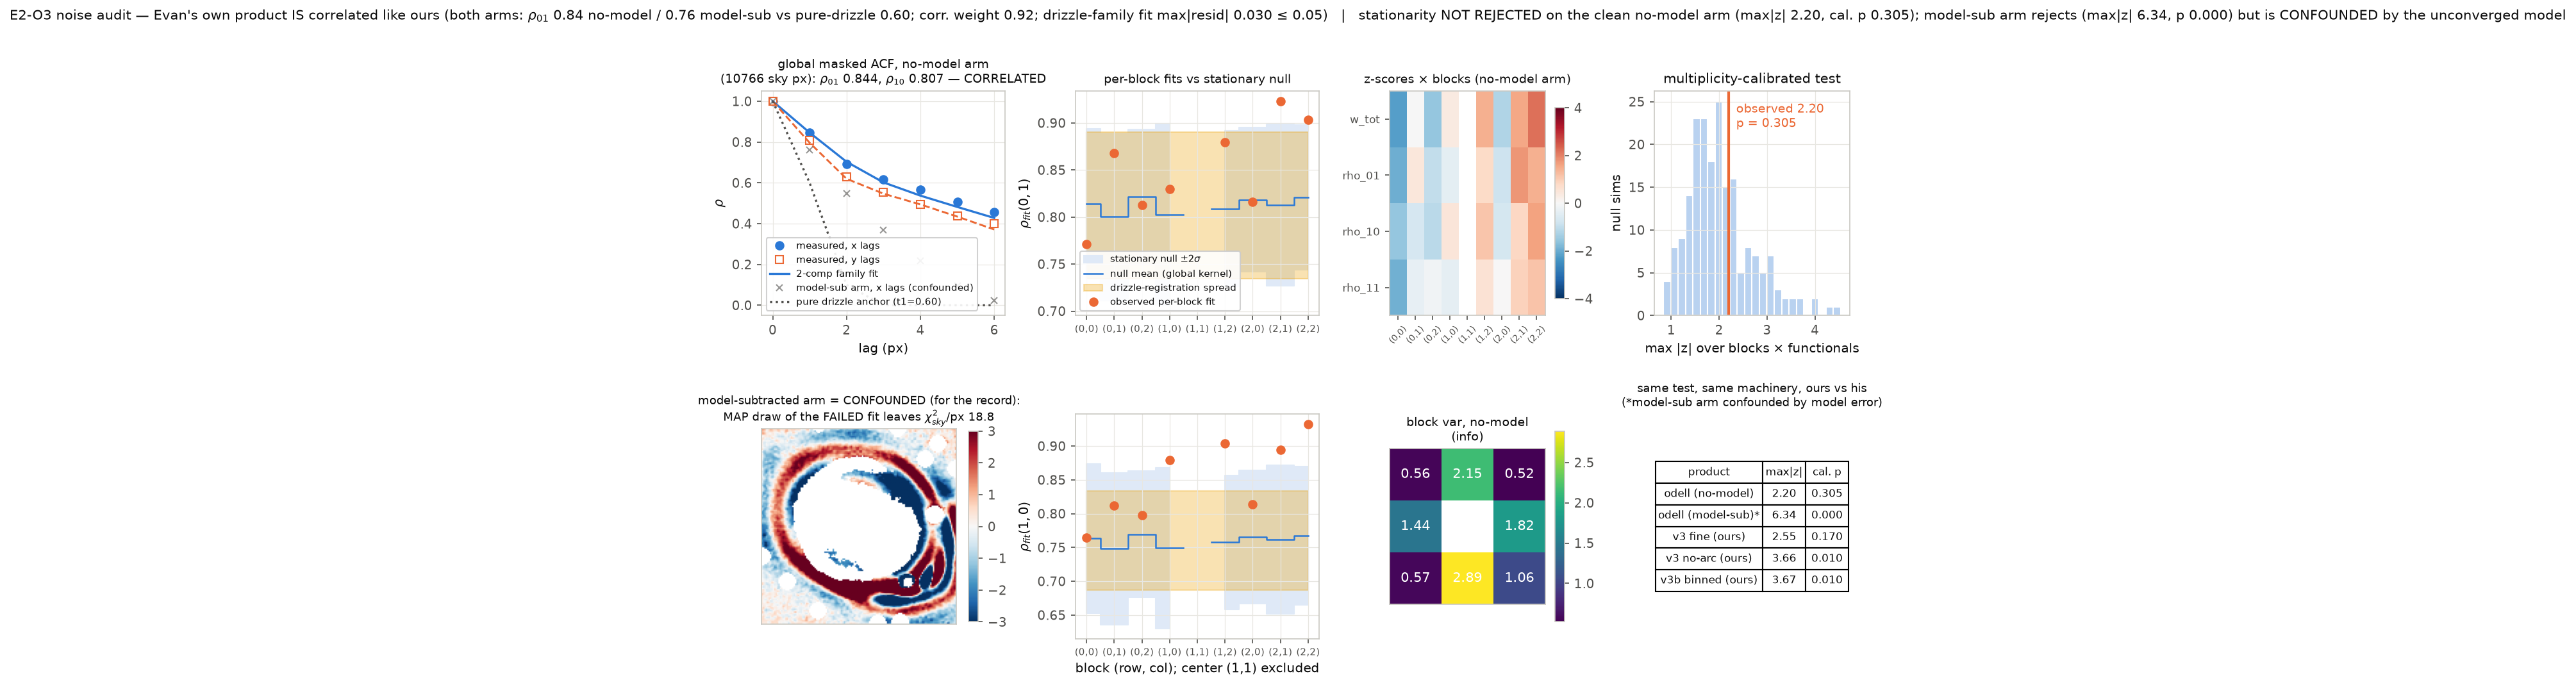
\includegraphics[width=0.98\textwidth]{../figs/e2_odell_noise.png}
\caption{The O3 noise audit of the collaborator's own product (T0.4-1
machinery; plotted before gate math). Top row, no-model arm: global
masked ACF over 10{,}766 sky pixels against the two-component
drizzle-family fit and the pure-drizzle anchor ($t_1=0.60$); per-block
$\rho_{01}$ against the stationary null and the drizzle-registration
spread; per-block $z$-scores; and the multiplicity-calibrated test
(observed max$|z|$ 2.20, $p=0.305$ --- no rejection on the clean arm).
Bottom row: the model-subtracted arm is kept for the record but
\emph{confounded} --- the best available model (the failed E2 fit's
max-log-density draw) leaves sky $\chi^2/\mathrm{px}=18.8$, so its hard
rejection (max$|z|$ 6.34) measures model error; the summary table runs
the same test with the same machinery on our own products (fine $p=0.17$;
binned $p=0.010$, rejected). Source artifact:
\dfile{data/e2\_odell\_noise.json}.}
\label{fig:e2noise}
\end{figure}

\paragraph{The product-dependence synthesis, updated.}
E2 sharpens the E1 synthesis into a clean split by product family.
\emph{The native scale is well-behaved}: the \dfile{v2d} native diagonal
target has now passed the strictest convergence gates in this program
twice (the E1 fit; the O4 control), both times at the anchor family.
\emph{The resampled products migrate}: both resampled products of this
sky --- our $0.08''$ binned drizzle and his $0.064125''$ half-native
preparation, produced by two fully independent pipelines --- migrate
every chain from a physical-basin warm start to the same
$\gammaEPL\approx1.10$ shelf under the plain diagonal likelihood, in
every seed group (128 of 128 chains across the two products), and the
correlated-likelihood money fit sits on the same shelf. Whatever the
mechanism's final form (the T0.4 stationarity rejection is its
noise-side face, \S\ref{sec:t041}), it travels with \emph{resampling of
this data}, not with any one pipeline, likelihood class, or sampler ---
and the native-scale anchor family ($1.4330$ old stack; $1.4683$
scene-API MCLMC) remains the only convergence-certified answer on this
sky.

\subsection{What it opens}

The honest open list is long, and most of it is deliberate non-spend
recorded in the gate ledger rather than silent omission.
{\bf Data-side injections}: the T1.1 injection-recovery test came back
confounded --- the control arm failed high {\it and} sick, implicating the
injection construction (scene-subtraction residue) under the pre-registered
honesty clause --- and the fit-side rescue (T1.1b) failed its entry gate
with an 85.8\% whitened-dof loss. Residue-free injections must be built on
the data side (kernel-sampled noise-only fields, sky-patch bootstrap, or
deeper multi-start subtraction); the mechanism's confirmatory test is
therefore still unrun, with one directional datum in its favor (same-data
corr$-$diag differential $-0.0526$, no defensible error bar).
{\bf The two-stage port}: a converged scene-substrate posterior on the
cond-$10^{14}$ target needs the two-stage re-preconditioning recipe ported
($\sim$0.5 day + 2--4 A100-h, estimated, not spent); until then ``the 1.433
anchor reproduces at posterior level on the new substrate'' is untested.
{\bf The locally-stationary whitener class}: the rejected stationary class
needs a successor; the ported likelihood deliberately keeps a pluggable
whitener seam for it, and the kernel-scan arm (E3) that would inform it
was deferred by plan and never funded --- it lapses at program close as
the standing caveat on absolute-$\gammaEPL$ claims. {\bf L1/L2 never ran}:
there is {\it no} production-SMC coverage certificate (L1) and no
supersampling/sub-pixel-PSF decomposition (L2); nothing in this report
should be read as implying either exists. {\bf PSF marginalization was
promoted and then never built} (its pool was reallocated by a later
decision); the D7 promotion language should not be read as delivered work.
The B4 preconditioning question (does per-$\lambda$ ensemble
preconditioning replace the two-stage recipe at cond-$10^{14}$?) closed
not-evaluable-within-budget and is genuinely open.

\subsection{Guidance for practitioners}

The decision matrix compresses to four rules. (1) If you need {\bf
evidence or mode structure} --- \logZ, basin weights, cold-start
robustness --- on targets up to the 74-d bimodal class, \mcsmc\ is the
vehicle, at single-digit A100-hours per basin; take the evidence error
from seed repeats, not from the per-run bootstrap (finding A). (2) If you
need a {\bf posterior on a carousel-class real multi-plane system}, budget
an order of magnitude more than we did or use a warm-started method and
accept the cold-start blind spot: at $\lesssim$16 A100-h {\it neither}
family converges (B1r). (3) Use {\bf MCLMC as a diagnostic}, freely --- and
never as the evidence kernel without Metropolis adjustment or a measured
bias budget. (4) {\bf Certify your references}: before freezing an
MCMC-derived posterior or evidence reference into an acceptance gate,
demand a coverage certificate at the gate's own $\sigma$-scale (findings
B; B3's blocked-by-reference row; the X2 frozen-set question). Our own
frozen reference failed this standard at $11\sigma$-equivalent scale ---
the most expensive single lesson of the campaign, and one we incurred
against ourselves.

\subsection{Operational lessons}

Four ops findings each cost real budget once and are now protocol.
{\bf (1) Pin the high-memory GPUs and re-measure after remat changes}: two
independent OOM failures (an injection arm on a 40-GB node, 1.49\,h
burned; the arbitration's 21-GiB single mutate allocation) traced to
memory sizings measured {\it with} rematerialization active and applied to
runs without it --- memory figures do not transfer across remat settings;
the fix is a hardware constraint pin plus fresh sizing. {\bf (2) The
scheduler snapshots scripts at submission}: a fix ``resubmitted'' after
editing the batch script re-ran the old code (two failed attempts);
protocol now verifies the {\it submitted} snapshot's checksum against the
intended file before trusting any resubmission. {\bf (3) One writer per
manifest}: concurrent session fronts clobbered the deploy checksum
manifest; the rule is pull-remote-first, union-merge, single writer per
wave. {\bf (4) Checkpoint everything}: the first production wave burned
94\% of its hours with zero artifacts (18.7\,h spent, 1.1\,h readable) ---
jobs died at walls holding all state in memory. The mid-campaign
checkpoint retrofit (per-stage full-state checkpoints, a graceful
wall-cap exit protocol distinguishing PARTIAL from crash, bit-identical
resume including the full \logZ\ bootstrap state, gated by a 58-test
suite) converted that failure mode into three-of-four readable recoveries,
and is the only reason the 12-hour carousel chain and every
$\lambda$-progress readout in Table~\ref{tab:decision} exist at all.
Smaller pins that will save a future campaign a day each: chunked mutation
sizes must divide {\it both} the particle count and the pilot subset; a
watchdog state for ``completed without artifact'' doubles as the harvest
reminder; BLAS thread caps matter on aarch64 login nodes; and the lensing
likelihood is never run on CPU.

%%%%%%%%%%%%%%%%%%%%%%%%%%%%%%%%%%%%%%%%%%%%%%%%%%%%%%%%%%%%%%%%%%%%%%%%%%%%%%%
\section{Reproducibility}
\label{sec:repro}
%%%%%%%%%%%%%%%%%%%%%%%%%%%%%%%%%%%%%%%%%%%%%%%%%%%%%%%%%%%%%%%%%%%%%%%%%%%%%%%

\paragraph{Ledgers and provenance.} The authoritative record is
\dfile{CAMPAIGN.md}: nine locked decisions (D1--D9), the A100-hour ledger
(rows appended {\it before} results are read, failed and zero-artifact jobs
counted in full), the gate record, and a dated stage log. Every gate ever
registered --- including the six that ended without a run and one
promoted-then-unbuilt item --- has a final disposition in
\dfile{research/gate\_ledger\_final.md}; nothing lapses silently. Among
the never-run items, two of our own programmed arms are named
explicitly: the S7 flow-preconditioned-MAMS arm (prerequisite unmet ---
the B1 $\lambda{=}1$ ensemble it required never came to exist) and the
X3 evidence-scored Vela-ladder prototype (never mobilized). Two
additional internal-reference benchmark arms were omitted under the
campaign's pre-declared external-collaboration bright line and are
dispositioned in the same ledger. Every
number in this report traces to an on-disk artifact via
\dfile{research/synthesis\_tables.md}, whose seven discrepancy flags
(artifact vs.\ ledger prose) are binding on this text: wherever the two
disagree the artifact value is quoted (e.g.\ the MCLMC demotion screen is
$20.1\sigma$ by \dfile{data/smc\_b0\_report.json}, not the ledger's
``$30\sigma$''; the L4 arbitration leg's on-disk record is
$\lambda=0.4183$ at a 12.26-h resume leg, with the ledger's
$\lambda\approx0.45$/18-h figure including earlier checkpointed legs). The
external claims register is \dfile{papers/handoff/CLAIMS.md}
(\S\ref{sec:gifts:handoff}). External release of this report is gated on
the sign-off checklist \dfile{papers/handoff/SIGNOFF\_CHECKLIST.md},
which lists the six passages characterizing unpublished upstream code
state that require the team's sign-off (internal use is unaffected; the
sixth passage is the E1 epilogue's description of the vendored
experimental MCLMC driver, \S\ref{sec:modelers} item~3).

\paragraph{Pre-registration discipline.} Every experimental cell was
pre-registered: a design checkpoint with hypothesis, predicted direction
and magnitude, falsifier, and derived thresholds, logged before
submission; figures plotted before gate text was written; amendments
(B1-reduced descope, the S6br budget-match, the B2$'$ re-registration)
ledgered as dated decisions with checksummed checkpoints, never edited in
place. Proposer and grader are separated throughout: every externally
relevant verdict in this report is {\it proposed (UNCERTIFIED ---
external)}, with certification belonging to the receiving team, and
scene-substrate results are labeled ``reproduced/measured, UNCERTIFIED
(external)'' --- ``validated'' is reserved for the old certified stack.

\paragraph{Environment freezes.} The campaign venv pins
python~3.13, \texttt{jax}/\texttt{jaxlib}~0.6.2, \texttt{blackjax}~1.3,
\texttt{tfp}~0.25.0, \texttt{numpy}~2.4.6 (a declared deviation from the
upstream 2.1.3 pin, covered by the gate battery), no
\texttt{tensorflow}; all installs pass \texttt{-c constraints.txt}. The
substrate is a vendored, {\it unpatched} snapshot of the upstream
development branch (full SHA in \dfile{VENDORED\_REF.txt}; the three
convention reconciliations live on our side of the seam), and the old
validated stack is imported by path at its certified ref. The
Perlmutter-native environment re-passed the full parity battery (F8, job
55980038) with the phoenix-side F1 value bit-consistent. Production
deploys are non-git rsync copies audited file-by-file against a checksum
manifest (225 files at close) before every submission.

\paragraph{Compute.} Table~\ref{tab:budget} is the phase budget against
actuals: {\bf 53.51 of 100 A100-h} at program close, nothing in flight
(per-row \texttt{sacct} rounding makes the component sum 53.52; flagged,
not smoothed). Free-tier phoenix spend (not A100): 12.38 L4 GPU-h (B3),
$\sim$29 A16-h (X2), and --- after program close --- the E1 epilogue's
9.56 L4-h (\S\ref{sec:modelers}) plus the E2 epilogue's 6.82 L4-h
(\S\ref{sec:e2}). Zero-artifact and failed jobs are counted at
full cost in their phases; the wave-1 post-mortem and the recovery-lane
economics are part of the record, not an embarrassment to be netted out.

\begin{table}[tbp]
\centering
\caption{A100-hour budget by phase: caps vs.\ ledgered actuals
(\dfile{CAMPAIGN.md} ledger; per-row \texttt{sacct}, Elapsed $\times$ 1
GPU, shared QOS). T1.1 was funded from the pool freed by D7's retirement
of P4; P2b by the D8 reallocation (10\,h freed-P4 + 8\,h stretch). The
100-h hard stop was never approached.}
\label{tab:budget}
\small
\begin{tabular}{@{}llrr@{}}
\toprule
phase & scope & cap [h] & actual [h] \\
\midrule
P0 & scaffold, parity gates F1--F8, SMC correctness (B0) & 1 & 0.00 \\
P1 & certification slice (T0.2/T0.3/T0.4) & 10 & 2.21 \\
T1.1 & injection-recovery on real drizzle noise (D7 pool) & 10 & 7.80 \\
P2 & sampler benchmark (B1--B5 waves + recovery lane) & 24 & 22.45 \\
P2b & carousel B1-reduced (S1r + S6br; D8/D9) & 18 & 15.85 \\
P3 & scene-substrate payload (L0, arbitration, L0-G2) & 17 & 5.21 \\
P4 & profile-class fork (retired at entry gate X1-G0) & 10 & 0.00 \\
\midrule
\multicolumn{2}{@{}l}{campaign total (hard stop 100)} & 100 & {\bf 53.51} \\
\bottomrule
\end{tabular}
\end{table}

\begin{figure}[htbp]
\centering
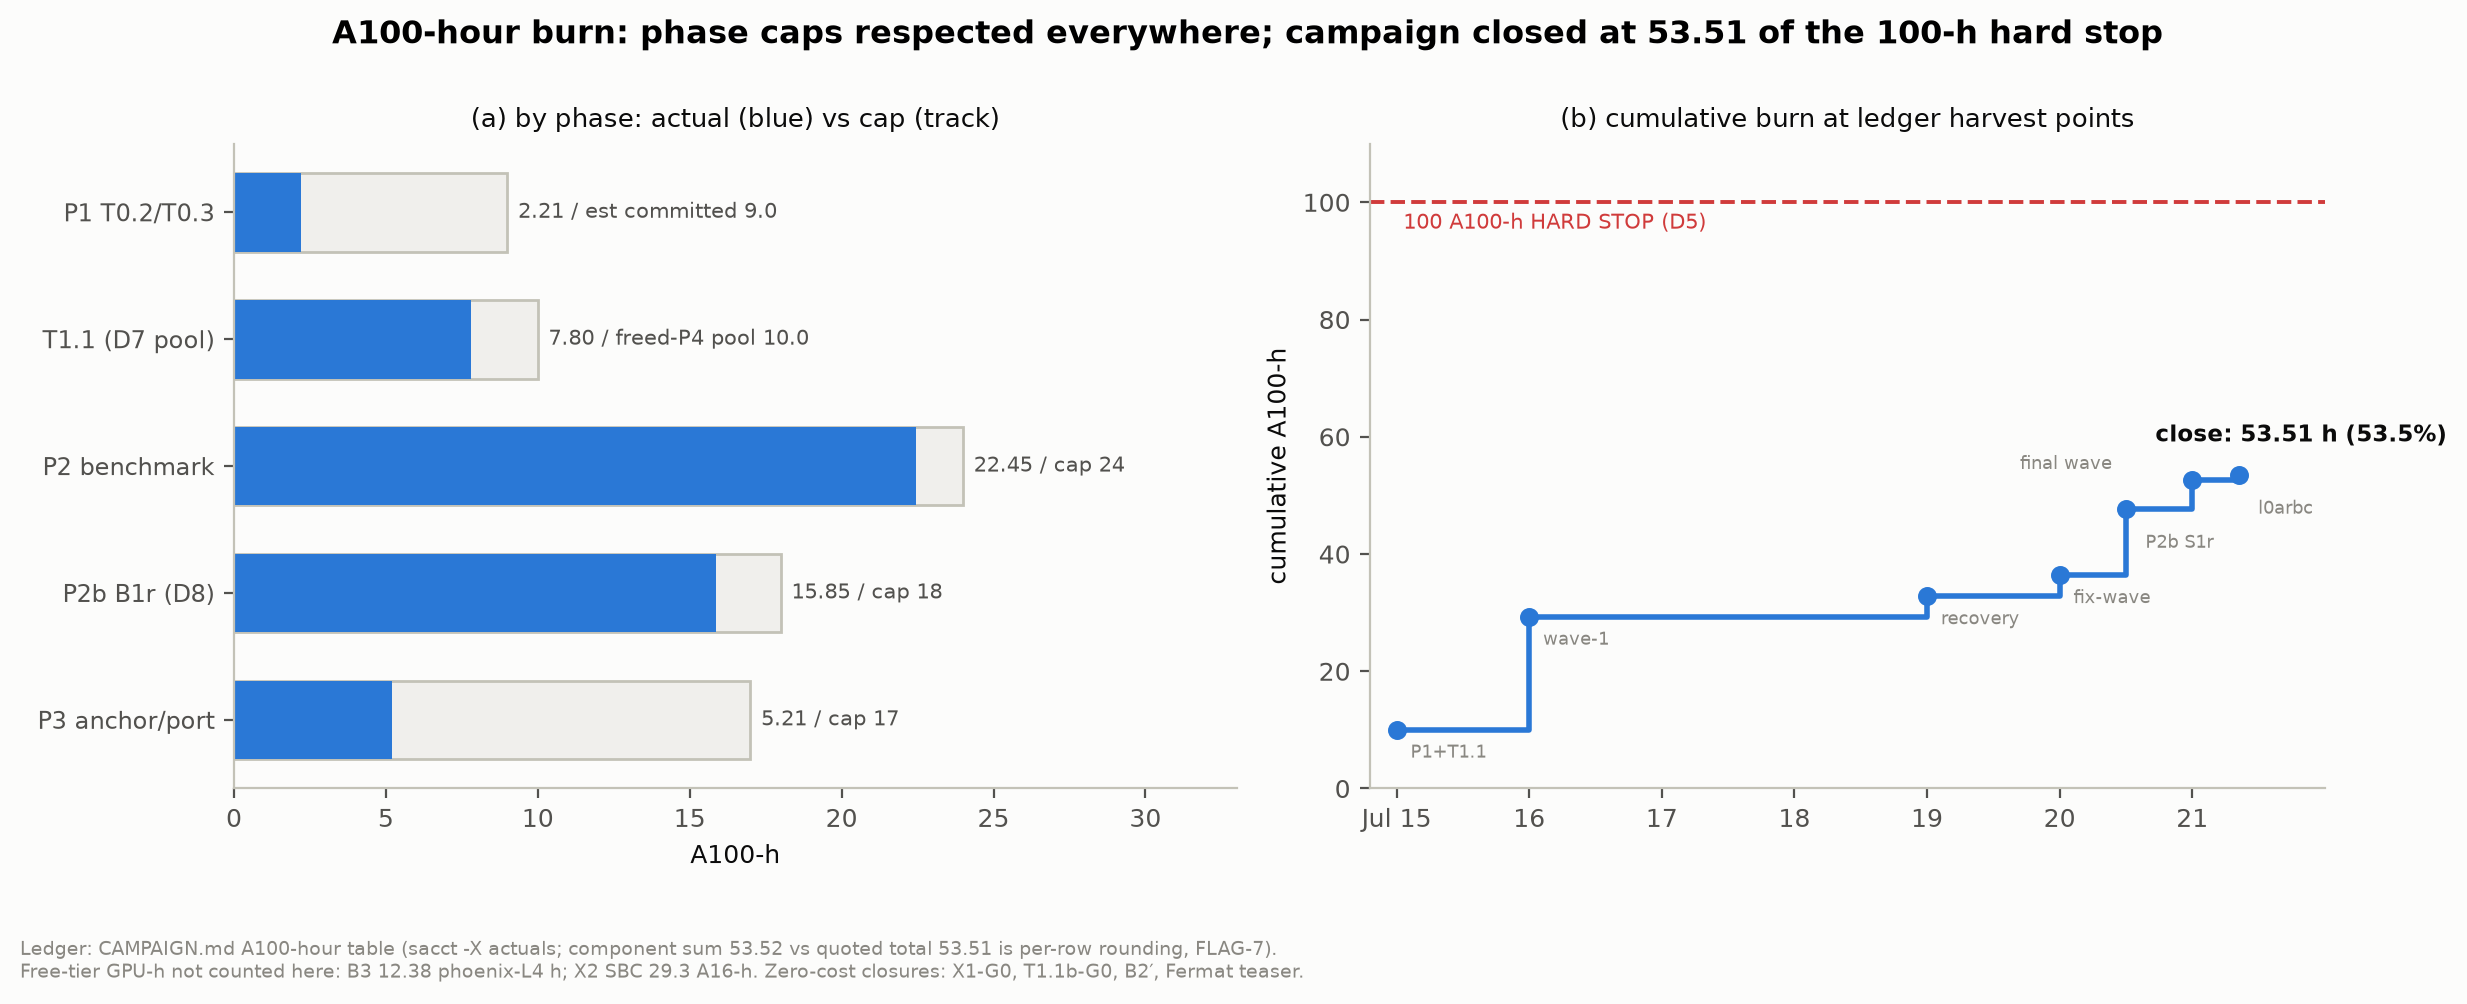
\includegraphics[width=0.98\textwidth]{../figs/rfig_budget_burn.png}
\caption{A100-hour burn. (a) Actual vs.\ cap by phase --- every fence
respected (P1 2.21, T1.1 7.80 of the D7-freed 10-h pool, P2 22.45/24,
P2b 15.85/18, P3 5.21/17). (b) Cumulative burn at the ledger's harvest
points (events in ledger order; sub-day $x$-offsets are display-only),
closing at \textbf{53.51} of the 100-h hard stop; the 53.52 component
sum is per-row \texttt{sacct} rounding (flagged, not smoothed).
Free-tier GPU-h (B3: 12.38 L4-h; X2: 29.3 A16-h) are additional and
uncounted here. Zero-cost closures: X1-G0, T1.1b, B2$'$, the Fermat
teaser. Source: \dfile{CAMPAIGN.md} A100-hour ledger
(append-before-read protocol).}
\label{fig:budget}
\end{figure}

\paragraph{Rebuilding the results.} The parity battery is
\dfile{01\_parity\_scene.py} (gates frozen in the README at P0); the SMC
correctness gates are \dfile{04\_smc\_micro\_validation.py}; each
benchmark cell names its runner, slurm script, seed, and artifact in its
ledger row; and each gate evaluation is a standalone JSON under
\dfile{data/} (Perlmutter production artifacts under
\dfile{data/results-perlmutter/}). The report builds with
\texttt{make -C papers pdf} against the shared
\dfile{reproductions/tech-report.sty} preamble.

%%%%%%%%%%%%%%%%%%%%%%%%%%%%%%%%%%%%%%%%%%%%%%%%%%%%%%%%%%%%%%%%%%%%%%%%%%%%%%%
%% end sections C
%%%%%%%%%%%%%%%%%%%%%%%%%%%%%%%%%%%%%%%%%%%%%%%%%%%%%%%%%%%%%%%%%%%%%%%%%%%%%%%
